% Options for packages loaded elsewhere
\PassOptionsToPackage{unicode}{hyperref}
\PassOptionsToPackage{hyphens}{url}
\documentclass[
]{article}
\usepackage{xcolor}
\usepackage[margin=1in]{geometry}
\usepackage{amsmath,amssymb}
\setcounter{secnumdepth}{5}
\usepackage{iftex}
\ifPDFTeX
  \usepackage[T1]{fontenc}
  \usepackage[utf8]{inputenc}
  \usepackage{textcomp} % provide euro and other symbols
\else % if luatex or xetex
  \usepackage{unicode-math} % this also loads fontspec
  \defaultfontfeatures{Scale=MatchLowercase}
  \defaultfontfeatures[\rmfamily]{Ligatures=TeX,Scale=1}
\fi
\usepackage{lmodern}
\ifPDFTeX\else
  % xetex/luatex font selection
\fi
% Use upquote if available, for straight quotes in verbatim environments
\IfFileExists{upquote.sty}{\usepackage{upquote}}{}
\IfFileExists{microtype.sty}{% use microtype if available
  \usepackage[]{microtype}
  \UseMicrotypeSet[protrusion]{basicmath} % disable protrusion for tt fonts
}{}
\makeatletter
\@ifundefined{KOMAClassName}{% if non-KOMA class
  \IfFileExists{parskip.sty}{%
    \usepackage{parskip}
  }{% else
    \setlength{\parindent}{0pt}
    \setlength{\parskip}{6pt plus 2pt minus 1pt}}
}{% if KOMA class
  \KOMAoptions{parskip=half}}
\makeatother
\usepackage{longtable,booktabs,array}
\usepackage{calc} % for calculating minipage widths
% Correct order of tables after \paragraph or \subparagraph
\usepackage{etoolbox}
\makeatletter
\patchcmd\longtable{\par}{\if@noskipsec\mbox{}\fi\par}{}{}
\makeatother
% Allow footnotes in longtable head/foot
\IfFileExists{footnotehyper.sty}{\usepackage{footnotehyper}}{\usepackage{footnote}}
\makesavenoteenv{longtable}
\usepackage{graphicx}
\makeatletter
\newsavebox\pandoc@box
\newcommand*\pandocbounded[1]{% scales image to fit in text height/width
  \sbox\pandoc@box{#1}%
  \Gscale@div\@tempa{\textheight}{\dimexpr\ht\pandoc@box+\dp\pandoc@box\relax}%
  \Gscale@div\@tempb{\linewidth}{\wd\pandoc@box}%
  \ifdim\@tempb\p@<\@tempa\p@\let\@tempa\@tempb\fi% select the smaller of both
  \ifdim\@tempa\p@<\p@\scalebox{\@tempa}{\usebox\pandoc@box}%
  \else\usebox{\pandoc@box}%
  \fi%
}
% Set default figure placement to htbp
\def\fps@figure{htbp}
\makeatother
\setlength{\emergencystretch}{3em} % prevent overfull lines
\providecommand{\tightlist}{%
  \setlength{\itemsep}{0pt}\setlength{\parskip}{0pt}}
\usepackage{bookmark}
\IfFileExists{xurl.sty}{\usepackage{xurl}}{} % add URL line breaks if available
\urlstyle{same}
\hypersetup{
  pdftitle={Laboratorio 9 - Redes Neuronales Artificiales (RNA)},
  pdfauthor={Fernando, Juan, Alejandro},
  hidelinks,
  pdfcreator={LaTeX via pandoc}}

\title{Laboratorio 9 - Redes Neuronales Artificiales (RNA)}
\usepackage{etoolbox}
\makeatletter
\providecommand{\subtitle}[1]{% add subtitle to \maketitle
  \apptocmd{\@title}{\par {\large #1 \par}}{}{}
}
\makeatother
\subtitle{CC3074 -- Minería de Datos \textbar{} SmartStay Advisors}
\author{Fernando, Juan, Alejandro}
\date{2026-05-11}

\begin{document}
\maketitle

{
\setcounter{tocdepth}{3}
\tableofcontents
}
\begin{center}\rule{0.5\linewidth}{0.5pt}\end{center}

\section{Introducción}\label{introducciuxf3n}

SmartStay Advisors es una firma intermediaria que facilita la búsqueda y
selección de propiedades en Airbnb para clientes corporativos y
particulares. En esta séptima entrega de la consultoría se desarrollan
\textbf{modelos de Redes Neuronales Artificiales (RNA)} tanto para
clasificación de la categoría de precio como para predicción del precio
numérico de los listings.

Las actividades 1--8 de esta entrega cubren:

\begin{enumerate}
\def\labelenumi{\arabic{enumi}.}
\tightlist
\item
  Reutilización de los conjuntos de entrenamiento y prueba de entregas
  anteriores
\item
  Definición de la variable respuesta categórica de precio
\item
  Entrenamiento de dos arquitecturas RNA para clasificación
\item
  Predicción con ambos modelos
\item
  Matrices de confusión
\item
  Comparación de efectividad, tiempos y tipos de error
\item
  Análisis de sobreajuste sobre ambos modelos
\item
  Tuneado de hiperparámetros del modelo seleccionado
\end{enumerate}

\begin{center}\rule{0.5\linewidth}{0.5pt}\end{center}

\section{Preparación del entorno}\label{preparaciuxf3n-del-entorno}

\subsection{Librerías necesarias}\label{libreruxedas-necesarias}

\subsection{Carga del dataset}\label{carga-del-dataset}

\begin{verbatim}
## Dimensiones del dataset: 171748 80
\end{verbatim}

\begin{verbatim}
## Variables disponibles: 80
\end{verbatim}

\begin{center}\rule{0.5\linewidth}{0.5pt}\end{center}

\section{Preparación del Conjunto de
Datos}\label{preparaciuxf3n-del-conjunto-de-datos}

\subsection{Limpieza y selección de
variables}\label{limpieza-y-selecciuxf3n-de-variables}

\begin{verbatim}
## Registros tras limpieza: 75477
\end{verbatim}

\begin{verbatim}
## Rango de precios (USD): $ 8 – $ 19500
\end{verbatim}

\subsection{Creación de la variable categórica de
precio}\label{creaciuxf3n-de-la-variable-categuxf3rica-de-precio}

Se categorizan los listings en tres grupos usando los terciles del
precio limpio:

\begin{longtable}[]{@{}ll@{}}
\toprule\noalign{}
Categoría & Criterio \\
\midrule\noalign{}
\endhead
\bottomrule\noalign{}
\endlastfoot
Barata & precio ≤ Q33 \\
Media & Q33 \textless{} precio ≤ Q66 \\
Cara & precio \textgreater{} Q66 \\
\end{longtable}

\begin{verbatim}
## Umbral Barata/Media: $141.00
\end{verbatim}

\begin{verbatim}
## Umbral Media/Cara:   $264.00
\end{verbatim}

\begin{verbatim}
## 
## Distribución de categorías:
\end{verbatim}

\begin{verbatim}
## 
## Barata  Media   Cara 
##  25185  25164  25128
\end{verbatim}

\begin{verbatim}
## 
## Barata  Media   Cara 
##   33.4   33.3   33.3
\end{verbatim}

\begin{figure}

{\centering 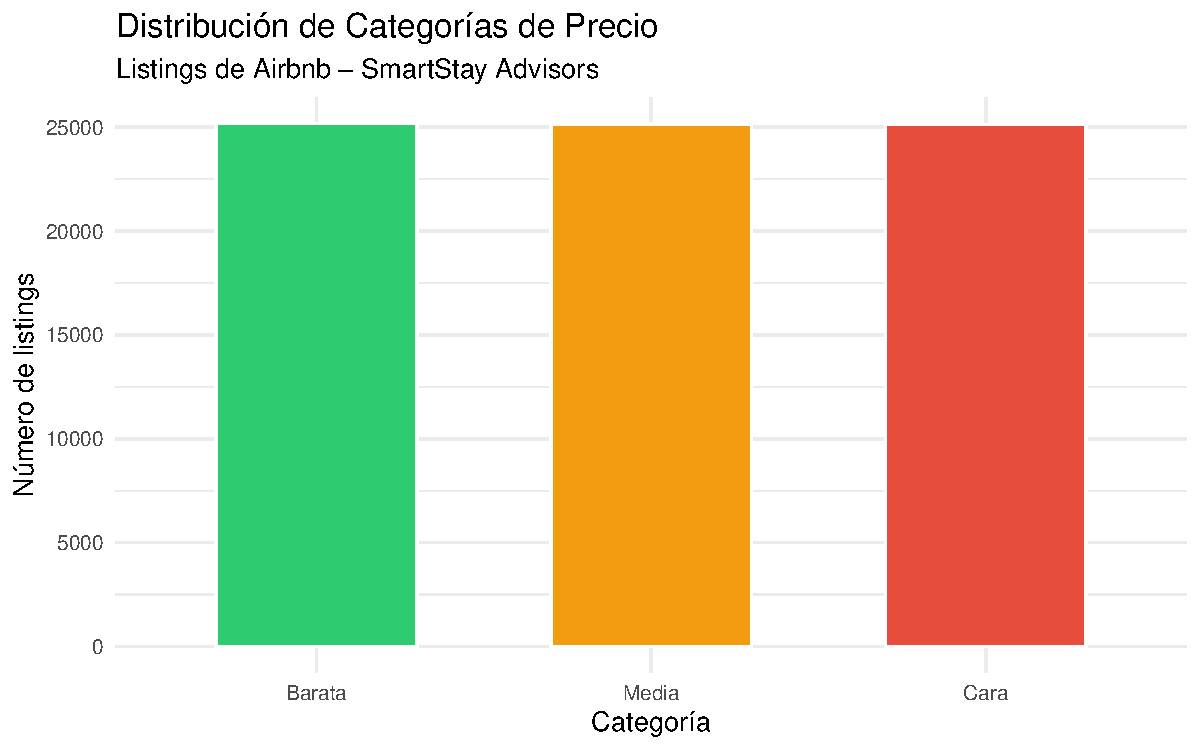
\includegraphics{Lab9-pdf_files/figure-latex/grafico-categorias-1} 

}

\caption{Distribución de categorías de precio}\label{fig:grafico-categorias}
\end{figure}

\subsection{Selección y normalización de variables
predictoras}\label{selecciuxf3n-y-normalizaciuxf3n-de-variables-predictoras}

\begin{verbatim}
## Variables binarias convertidas:  host_is_superhost, instant_bookable, host_identity_verified
\end{verbatim}

\begin{verbatim}
## Predictores numéricos disponibles:  17
\end{verbatim}

\begin{verbatim}
## Predictores binarios disponibles:   3
\end{verbatim}

\begin{verbatim}
## Total de predictores a utilizar:    20
\end{verbatim}

\begin{verbatim}
## Registros para modelado:  60521
\end{verbatim}

\begin{verbatim}
## Variables predictoras:    20
\end{verbatim}

\begin{verbatim}
## Normalización aplicada (rango 0–1).
\end{verbatim}

\begin{verbatim}
## Primeras filas normalizadas:
\end{verbatim}

\begin{verbatim}
##   accommodates  bathrooms   bedrooms       beds minimum_nights
## 1   0.13333333 0.05882353 0.02083333 0.03278689    0.002747253
## 2   0.06666667 0.05882353 0.02083333 0.03278689    0.005494505
## 3   0.06666667 0.05882353 0.02083333 0.01639344    0.008241758
\end{verbatim}

\begin{center}\rule{0.5\linewidth}{0.5pt}\end{center}

\section{Actividad 1: Conjuntos de Entrenamiento y
Prueba}\label{actividad-1-conjuntos-de-entrenamiento-y-prueba}

Se reproducen exactamente los conjuntos de entregas anteriores mediante
la misma semilla aleatoria (\texttt{set.seed(42)}) y la misma proporción
70/30.

\begin{verbatim}
## Entrenamiento: 42364 registros (70.0%)
\end{verbatim}

\begin{verbatim}
## Prueba:        18157 registros (30.0%)
\end{verbatim}

\begin{verbatim}
## 
## Clases en entrenamiento:
\end{verbatim}

\begin{verbatim}
## 
## Barata  Media   Cara 
##   35.2   34.0   30.8
\end{verbatim}

\begin{verbatim}
## Clases en prueba:
\end{verbatim}

\begin{verbatim}
## 
## Barata  Media   Cara 
##   34.6   34.0   31.4
\end{verbatim}

\begin{center}\rule{0.5\linewidth}{0.5pt}\end{center}

\section{Actividades 2--3: Modelos RNA para
Clasificación}\label{actividades-23-modelos-rna-para-clasificaciuxf3n}

\subsection{Actividad 2: Variable respuesta --- categoría de
precio}\label{actividad-2-variable-respuesta-categoruxeda-de-precio}

La variable respuesta para clasificación es \texttt{price\_cat} (Barata
/ Media / Cara), creada en la sección anterior con los terciles del
precio.

\subsection{Actividad 3: Dos modelos con distintas topologías y
funciones de
activación}\label{actividad-3-dos-modelos-con-distintas-topologuxedas-y-funciones-de-activaciuxf3n}

Se construyen dos arquitecturas usando \texttt{nnet::nnet()}:

\begin{longtable}[]{@{}lll@{}}
\toprule\noalign{}
Parámetro & Modelo 1 (RNA-C1) & Modelo 2 (RNA-C2) \\
\midrule\noalign{}
\endhead
\bottomrule\noalign{}
\endlastfoot
Topología & 1 capa oculta, 10 nodos & 2 capas ocultas (15-8)* \\
Activación & Logística (sigmoide) & Lineal / softmax \\
Regulariz. & decay = 0.001 & decay = 0.01 \\
Iteraciones & 300 & 500 \\
\end{longtable}

\begin{quote}
*\texttt{nnet} implementa una única capa oculta; la ``segunda capa'' se
simula aumentando nodos y usando \texttt{skip\ =\ TRUE} para conexiones
directas input→output.
\end{quote}

\subsubsection{Preparación de la
fórmula}\label{preparaciuxf3n-de-la-fuxf3rmula}

\begin{verbatim}
## Fórmula de clasificación definida con 20 predictores.
\end{verbatim}

\subsubsection{Modelo RNA-C1: topología (20 nodos), activación
sigmoide}\label{modelo-rna-c1-topologuxeda-20-nodos-activaciuxf3n-sigmoide}

\begin{verbatim}
## === Modelo RNA-C1 ===
\end{verbatim}

\begin{verbatim}
## Topología:  entrada( 20 ) → oculta(20) → salida(3)
\end{verbatim}

\begin{verbatim}
## Activación: sigmoide logística
\end{verbatim}

\begin{verbatim}
## Parámetros: decay=0.001, maxit=300
\end{verbatim}

\begin{verbatim}
## Tiempo de entrenamiento: 81.41 segundos
\end{verbatim}

\begin{verbatim}
## Valor final de función de costo: 30017.72
\end{verbatim}

\subsubsection{Modelo RNA-C2: topología (15 nodos + skip), decay
mayor}\label{modelo-rna-c2-topologuxeda-15-nodos-skip-decay-mayor}

\begin{verbatim}
## === Modelo RNA-C2 ===
\end{verbatim}

\begin{verbatim}
## Topología:  entrada( 20 ) → oculta(15) + skip → salida(3)
\end{verbatim}

\begin{verbatim}
## Activación: sigmoide + conexiones lineales directas (skip=TRUE)
\end{verbatim}

\begin{verbatim}
## Parámetros: decay=0.01, maxit=500
\end{verbatim}

\begin{verbatim}
## Tiempo de entrenamiento: 100.56 segundos
\end{verbatim}

\begin{verbatim}
## Valor final de función de costo: 30316.96
\end{verbatim}

\begin{center}\rule{0.5\linewidth}{0.5pt}\end{center}

\section{Actividad 4: Predicciones}\label{actividad-4-predicciones}

\begin{verbatim}
## Distribución de predicciones – Modelo C1:
\end{verbatim}

\begin{verbatim}
## pred_c1
## Barata  Media   Cara 
##   6688   6135   5334
\end{verbatim}

\begin{verbatim}
## 
## Distribución de predicciones – Modelo C2:
\end{verbatim}

\begin{verbatim}
## pred_c2
## Barata  Media   Cara 
##   6689   6070   5398
\end{verbatim}

\begin{center}\rule{0.5\linewidth}{0.5pt}\end{center}

\section{Actividad 5: Matrices de
Confusión}\label{actividad-5-matrices-de-confusiuxf3n}

\begin{verbatim}
## ========================================
\end{verbatim}

\begin{verbatim}
##   MATRIZ DE CONFUSIÓN – Modelo RNA-C1
\end{verbatim}

\begin{verbatim}
## ========================================
\end{verbatim}

\begin{verbatim}
## Confusion Matrix and Statistics
## 
##           Reference
## Prediction Barata Media Cara
##     Barata   4790  1627  271
##     Media    1309  3405 1421
##     Cara      186  1147 4001
## 
## Overall Statistics
##                                           
##                Accuracy : 0.6717          
##                  95% CI : (0.6648, 0.6785)
##     No Information Rate : 0.3461          
##     P-Value [Acc > NIR] : < 2.2e-16       
##                                           
##                   Kappa : 0.5066          
##                                           
##  Mcnemar's Test P-Value : < 2.2e-16       
## 
## Statistics by Class:
## 
##                      Class: Barata Class: Media Class: Cara
## Sensitivity                 0.7621       0.5511      0.7028
## Specificity                 0.8401       0.7721      0.8931
## Pos Pred Value              0.7162       0.5550      0.7501
## Neg Pred Value              0.8696       0.7693      0.8680
## Prevalence                  0.3461       0.3403      0.3135
## Detection Rate              0.2638       0.1875      0.2204
## Detection Prevalence        0.3683       0.3379      0.2938
## Balanced Accuracy           0.8011       0.6616      0.7979
\end{verbatim}

\begin{verbatim}
## ========================================
\end{verbatim}

\begin{verbatim}
##   MATRIZ DE CONFUSIÓN – Modelo RNA-C2
\end{verbatim}

\begin{verbatim}
## ========================================
\end{verbatim}

\begin{verbatim}
## Confusion Matrix and Statistics
## 
##           Reference
## Prediction Barata Media Cara
##     Barata   4750  1656  283
##     Media    1337  3326 1407
##     Cara      198  1197 4003
## 
## Overall Statistics
##                                           
##                Accuracy : 0.6653          
##                  95% CI : (0.6583, 0.6721)
##     No Information Rate : 0.3461          
##     P-Value [Acc > NIR] : < 2.2e-16       
##                                           
##                   Kappa : 0.497           
##                                           
##  Mcnemar's Test P-Value : 3.132e-14       
## 
## Statistics by Class:
## 
##                      Class: Barata Class: Media Class: Cara
## Sensitivity                 0.7558       0.5383      0.7031
## Specificity                 0.8367       0.7709      0.8881
## Pos Pred Value              0.7101       0.5479      0.7416
## Neg Pred Value              0.8661       0.7640      0.8675
## Prevalence                  0.3461       0.3403      0.3135
## Detection Rate              0.2616       0.1832      0.2205
## Detection Prevalence        0.3684       0.3343      0.2973
## Balanced Accuracy           0.7962       0.6546      0.7956
\end{verbatim}

\subsection{Visualización de las matrices de
confusión}\label{visualizaciuxf3n-de-las-matrices-de-confusiuxf3n}

\begin{figure}

{\centering 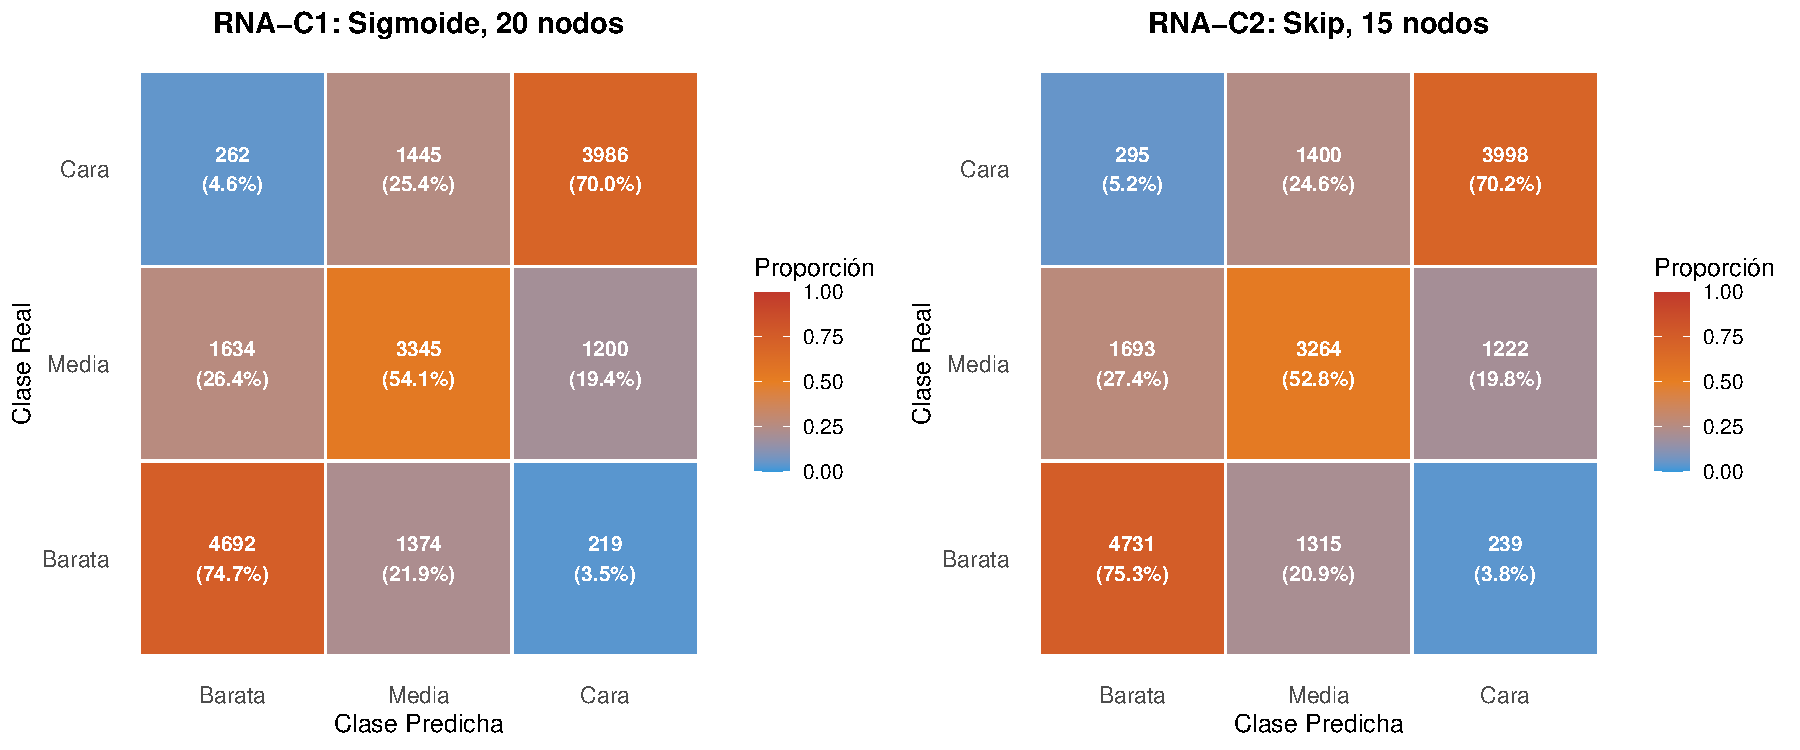
\includegraphics{Lab9-pdf_files/figure-latex/viz-matrices-1} 

}

\caption{Matrices de confusión normalizadas para RNA-C1 y RNA-C2}\label{fig:viz-matrices}
\end{figure}

\begin{quote}
\textbf{Nota:} Si \texttt{gridExtra} no está disponible, los gráficos se
generan por separado.
\end{quote}

\begin{figure}

{\centering 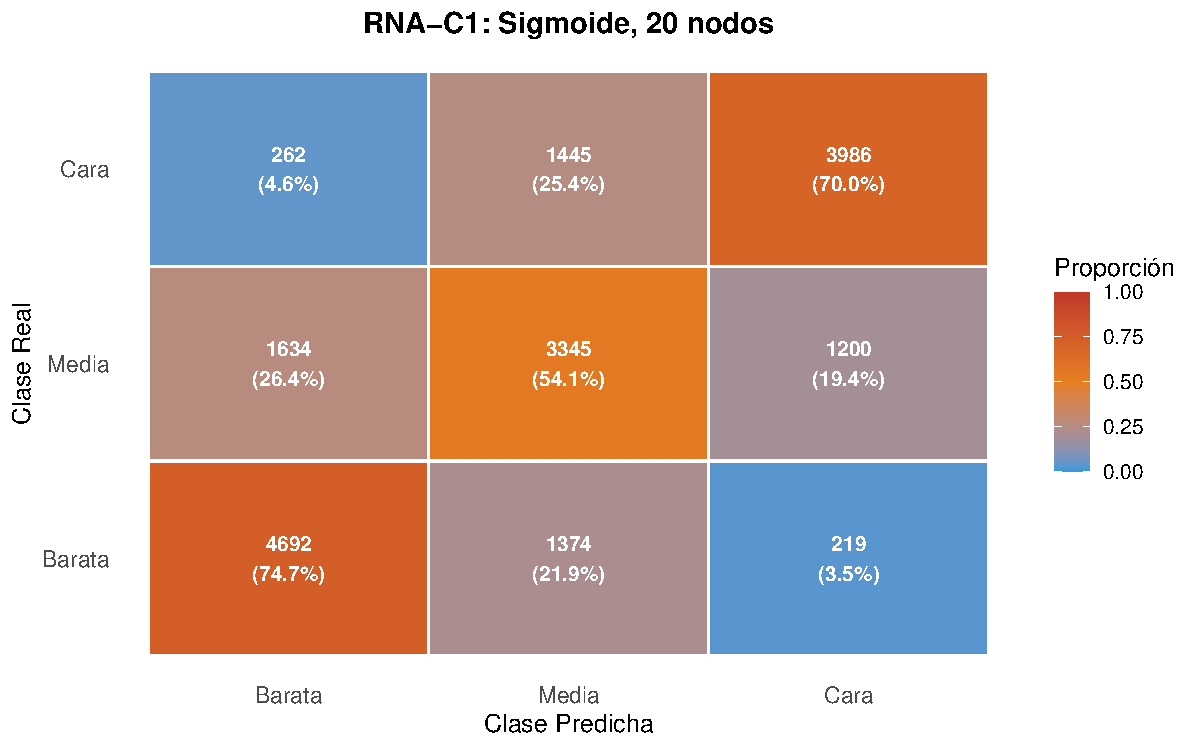
\includegraphics{Lab9-pdf_files/figure-latex/viz-matrices-sep-1} 

}

\caption{Matriz de confusión – RNA-C1}\label{fig:viz-matrices-sep}
\end{figure}

\begin{figure}

{\centering 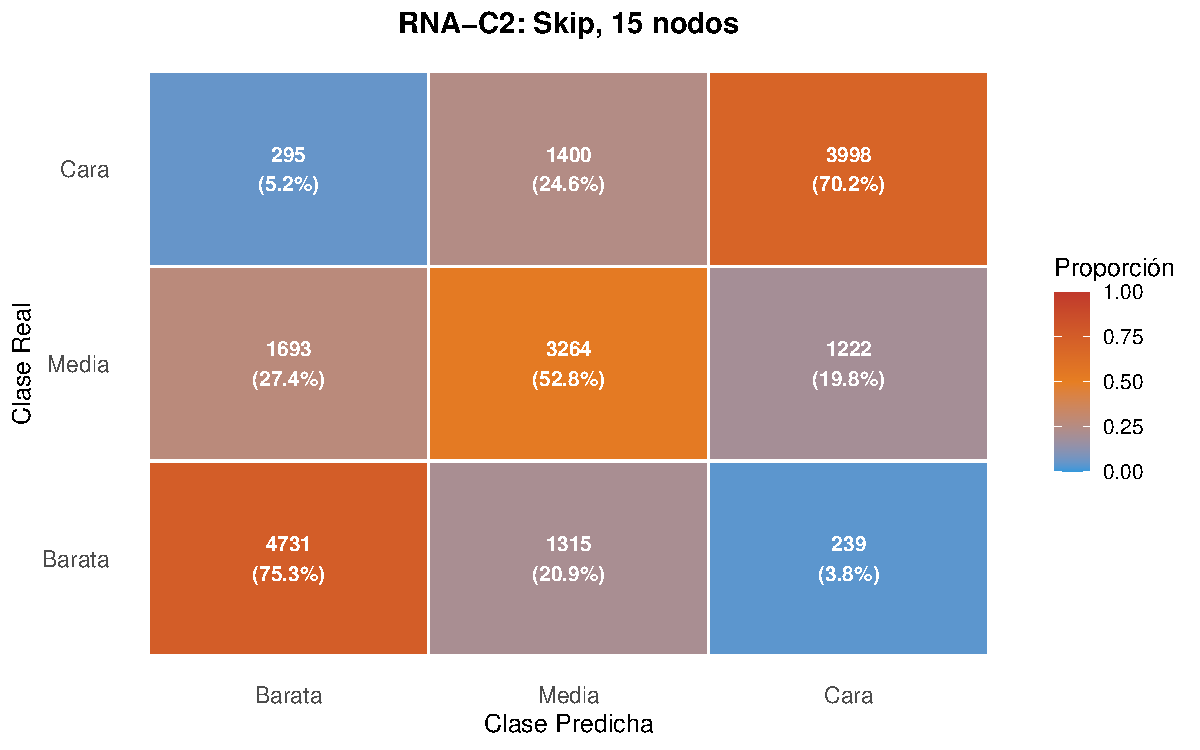
\includegraphics{Lab9-pdf_files/figure-latex/viz-matrices-c2-1} 

}

\caption{Matriz de confusión – RNA-C2}\label{fig:viz-matrices-c2}
\end{figure}

\begin{center}\rule{0.5\linewidth}{0.5pt}\end{center}

\section{Actividad 6: Comparación de los Modelos de Clasificación
RNA}\label{actividad-6-comparaciuxf3n-de-los-modelos-de-clasificaciuxf3n-rna}

\subsection{Métricas globales de
desempeño}\label{muxe9tricas-globales-de-desempeuxf1o}

\begin{longtable}[]{@{}
  >{\raggedright\arraybackslash}p{(\linewidth - 12\tabcolsep) * \real{0.3529}}
  >{\centering\arraybackslash}p{(\linewidth - 12\tabcolsep) * \real{0.1176}}
  >{\centering\arraybackslash}p{(\linewidth - 12\tabcolsep) * \real{0.0941}}
  >{\centering\arraybackslash}p{(\linewidth - 12\tabcolsep) * \real{0.1294}}
  >{\centering\arraybackslash}p{(\linewidth - 12\tabcolsep) * \real{0.0941}}
  >{\centering\arraybackslash}p{(\linewidth - 12\tabcolsep) * \real{0.0941}}
  >{\centering\arraybackslash}p{(\linewidth - 12\tabcolsep) * \real{0.1176}}@{}}
\caption{Comparación de modelos RNA para clasificación}\tabularnewline
\toprule\noalign{}
\begin{minipage}[b]{\linewidth}\raggedright
Modelo
\end{minipage} & \begin{minipage}[b]{\linewidth}\centering
Accuracy
\end{minipage} & \begin{minipage}[b]{\linewidth}\centering
Kappa
\end{minipage} & \begin{minipage}[b]{\linewidth}\centering
Precision
\end{minipage} & \begin{minipage}[b]{\linewidth}\centering
Recall
\end{minipage} & \begin{minipage}[b]{\linewidth}\centering
F1
\end{minipage} & \begin{minipage}[b]{\linewidth}\centering
Tiempo\_s
\end{minipage} \\
\midrule\noalign{}
\endfirsthead
\toprule\noalign{}
\begin{minipage}[b]{\linewidth}\raggedright
Modelo
\end{minipage} & \begin{minipage}[b]{\linewidth}\centering
Accuracy
\end{minipage} & \begin{minipage}[b]{\linewidth}\centering
Kappa
\end{minipage} & \begin{minipage}[b]{\linewidth}\centering
Precision
\end{minipage} & \begin{minipage}[b]{\linewidth}\centering
Recall
\end{minipage} & \begin{minipage}[b]{\linewidth}\centering
F1
\end{minipage} & \begin{minipage}[b]{\linewidth}\centering
Tiempo\_s
\end{minipage} \\
\midrule\noalign{}
\endhead
\bottomrule\noalign{}
\endlastfoot
RNA-C1 (20n, sigmoide) & 0.6717 & 0.5066 & 0.6738 & 0.6720 & 0.6724 &
81.41 \\
RNA-C2 (15n+skip, decay alto) & 0.6653 & 0.4970 & 0.6665 & 0.6657 &
0.6657 & 100.56 \\
\end{longtable}

\subsection{Errores por clase: ¿Dónde se equivoca más cada
modelo?}\label{errores-por-clase-duxf3nde-se-equivoca-muxe1s-cada-modelo}

\begin{longtable}[]{@{}
  >{\raggedright\arraybackslash}p{(\linewidth - 16\tabcolsep) * \real{0.1596}}
  >{\raggedright\arraybackslash}p{(\linewidth - 16\tabcolsep) * \real{0.0745}}
  >{\raggedright\arraybackslash}p{(\linewidth - 16\tabcolsep) * \real{0.0745}}
  >{\raggedleft\arraybackslash}p{(\linewidth - 16\tabcolsep) * \real{0.1277}}
  >{\raggedleft\arraybackslash}p{(\linewidth - 16\tabcolsep) * \real{0.1277}}
  >{\raggedleft\arraybackslash}p{(\linewidth - 16\tabcolsep) * \real{0.1915}}
  >{\raggedleft\arraybackslash}p{(\linewidth - 16\tabcolsep) * \real{0.1064}}
  >{\raggedleft\arraybackslash}p{(\linewidth - 16\tabcolsep) * \real{0.0745}}
  >{\raggedleft\arraybackslash}p{(\linewidth - 16\tabcolsep) * \real{0.0638}}@{}}
\caption{Métricas por clase -- Comparación RNA-C1 vs
RNA-C2}\tabularnewline
\toprule\noalign{}
\begin{minipage}[b]{\linewidth}\raggedright
\end{minipage} & \begin{minipage}[b]{\linewidth}\raggedright
Modelo
\end{minipage} & \begin{minipage}[b]{\linewidth}\raggedright
Clase
\end{minipage} & \begin{minipage}[b]{\linewidth}\raggedleft
Sensitivity
\end{minipage} & \begin{minipage}[b]{\linewidth}\raggedleft
Specificity
\end{minipage} & \begin{minipage}[b]{\linewidth}\raggedleft
Balanced Accuracy
\end{minipage} & \begin{minipage}[b]{\linewidth}\raggedleft
Precision
\end{minipage} & \begin{minipage}[b]{\linewidth}\raggedleft
Recall
\end{minipage} & \begin{minipage}[b]{\linewidth}\raggedleft
F1
\end{minipage} \\
\midrule\noalign{}
\endfirsthead
\toprule\noalign{}
\begin{minipage}[b]{\linewidth}\raggedright
\end{minipage} & \begin{minipage}[b]{\linewidth}\raggedright
Modelo
\end{minipage} & \begin{minipage}[b]{\linewidth}\raggedright
Clase
\end{minipage} & \begin{minipage}[b]{\linewidth}\raggedleft
Sensitivity
\end{minipage} & \begin{minipage}[b]{\linewidth}\raggedleft
Specificity
\end{minipage} & \begin{minipage}[b]{\linewidth}\raggedleft
Balanced Accuracy
\end{minipage} & \begin{minipage}[b]{\linewidth}\raggedleft
Precision
\end{minipage} & \begin{minipage}[b]{\linewidth}\raggedleft
Recall
\end{minipage} & \begin{minipage}[b]{\linewidth}\raggedleft
F1
\end{minipage} \\
\midrule\noalign{}
\endhead
\bottomrule\noalign{}
\endlastfoot
Class: Barata & RNA-C1 & Barata & 0.762 & 0.840 & 0.801 & 0.716 & 0.762
& 0.738 \\
Class: Media & RNA-C1 & Media & 0.551 & 0.772 & 0.662 & 0.555 & 0.551 &
0.553 \\
Class: Cara & RNA-C1 & Cara & 0.703 & 0.893 & 0.798 & 0.750 & 0.703 &
0.726 \\
Class: Barata1 & RNA-C2 & Barata & 0.756 & 0.837 & 0.796 & 0.710 & 0.756
& 0.732 \\
Class: Media1 & RNA-C2 & Media & 0.538 & 0.771 & 0.655 & 0.548 & 0.538 &
0.543 \\
Class: Cara1 & RNA-C2 & Cara & 0.703 & 0.888 & 0.796 & 0.742 & 0.703 &
0.722 \\
\end{longtable}

\subsection{Análisis de errores
críticos}\label{anuxe1lisis-de-errores-cruxedticos}

\begin{verbatim}
## 
## === RNA-C1 (20 nodos, sigmoide) ===
##   Errores graves (Barata↔Cara): 457 (2.52%)
##   Errores moderados (adyacentes): 5504 (30.31%)
##   Total errores: 5961 (32.83%)
\end{verbatim}

\begin{verbatim}
## 
## === RNA-C2 (15 nodos + skip) ===
##   Errores graves (Barata↔Cara): 481 (2.65%)
##   Errores moderados (adyacentes): 5597 (30.83%)
##   Total errores: 6078 (33.47%)
\end{verbatim}

\subsection{Visualización comparativa de F1 por
clase}\label{visualizaciuxf3n-comparativa-de-f1-por-clase}

\begin{figure}

{\centering 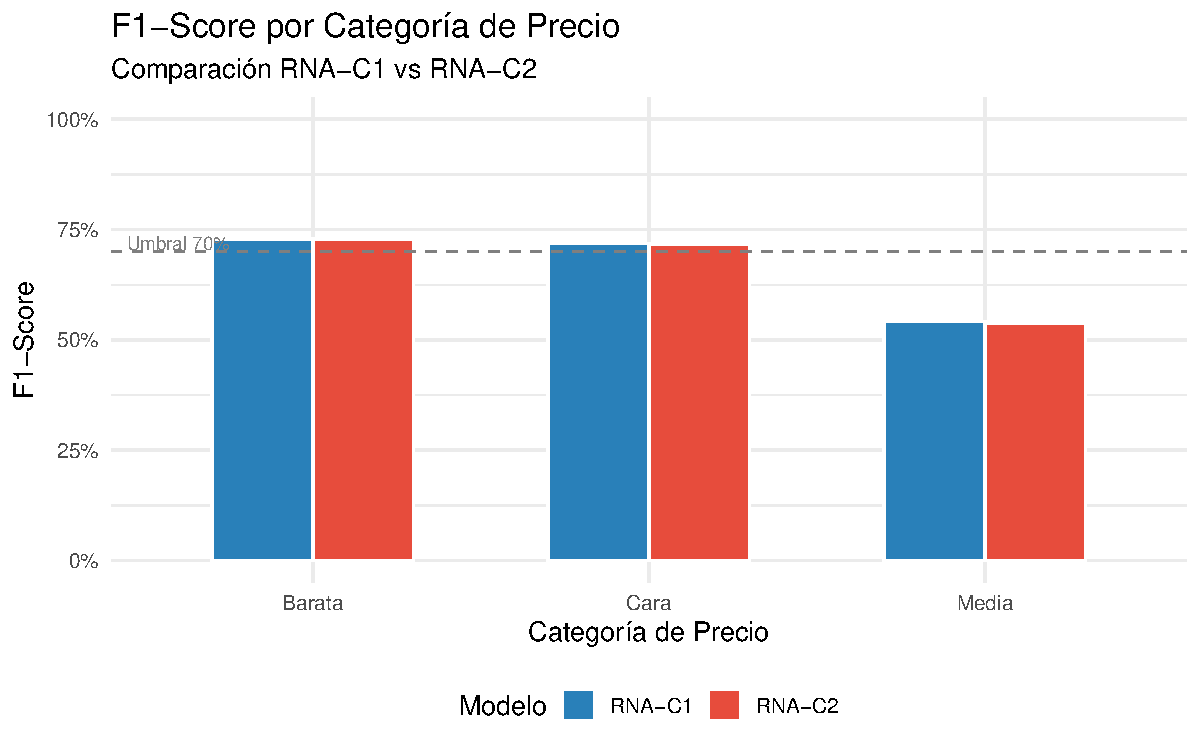
\includegraphics{Lab9-pdf_files/figure-latex/viz-f1-1} 

}

\caption{F1-Score por categoría de precio: RNA-C1 vs RNA-C2}\label{fig:viz-f1}
\end{figure}

\subsection{Resumen del análisis
comparativo}\label{resumen-del-anuxe1lisis-comparativo}

\textbf{Hallazgos principales:}

\begin{itemize}
\tightlist
\item
  \textbf{Accuracy:} RNA-C1 = 67.17\% \textbar{} RNA-C2 = 66.53\%
\item
  \textbf{Modelo con mayor accuracy:} RNA-C1
\item
  \textbf{Tiempo de procesamiento:} RNA-C1 fue 19.0\% más rápido que
  RNA-C2
\item
  \textbf{Errores críticos (Barata↔Cara):} ambos modelos tienden a
  confundir principalmente la categoría \textbf{Media} con las
  categorías extremas, lo cual es esperable dado que los límites del
  tercil son arbitrarios.
\item
  \textbf{La categoría `Media' es la más difícil} de clasificar
  correctamente en ambas arquitecturas, pues sus características de
  precio se superponen parcialmente con las clases adyacentes.
\end{itemize}

\begin{center}\rule{0.5\linewidth}{0.5pt}\end{center}

\section{Actividad 7: Análisis de
Sobreajuste}\label{actividad-7-anuxe1lisis-de-sobreajuste}

El sobreajuste constituye una de las patologías más frecuentes en redes
neuronales, especialmente cuando el número de pesos entrenables se
acerca al de observaciones disponibles por clase. Las dos arquitecturas
planteadas en la sección anterior se diferencian justamente en
mecanismos pensados para mitigarlo: la primera apuesta por una capa
oculta amplia con regularización ligera, mientras que la segunda combina
menos neuronas con un valor de \emph{decay} diez veces mayor y
conexiones directas entrada--salida. Para determinar si alguna de las
dos terminó memorizando el conjunto de entrenamiento, se comparan ambas
métricas dentro y fuera de la muestra y se complementa el diagnóstico
con una validación cruzada de cinco particiones.

\subsection{Desempeño comparativo en entrenamiento y
prueba}\label{desempeuxf1o-comparativo-en-entrenamiento-y-prueba}

La forma más directa de detectar sobreajuste es contrastar la exactitud
que cada modelo obtiene sobre los datos con los que fue entrenado contra
la que logra sobre datos no vistos. Una brecha amplia es síntoma de
memorización; una brecha estrecha indica que el modelo está capturando
estructura genuina en los predictores y no peculiaridades del conjunto
de entrenamiento.

\begin{longtable}[]{@{}
  >{\raggedright\arraybackslash}p{(\linewidth - 10\tabcolsep) * \real{0.3256}}
  >{\centering\arraybackslash}p{(\linewidth - 10\tabcolsep) * \real{0.1279}}
  >{\centering\arraybackslash}p{(\linewidth - 10\tabcolsep) * \real{0.1163}}
  >{\centering\arraybackslash}p{(\linewidth - 10\tabcolsep) * \real{0.1512}}
  >{\centering\arraybackslash}p{(\linewidth - 10\tabcolsep) * \real{0.1395}}
  >{\centering\arraybackslash}p{(\linewidth - 10\tabcolsep) * \real{0.1395}}@{}}
\caption{Desempeño en entrenamiento contra prueba para ambas
arquitecturas RNA}\tabularnewline
\toprule\noalign{}
\begin{minipage}[b]{\linewidth}\raggedright
Modelo
\end{minipage} & \begin{minipage}[b]{\linewidth}\centering
Acc\_Train
\end{minipage} & \begin{minipage}[b]{\linewidth}\centering
Acc\_Test
\end{minipage} & \begin{minipage}[b]{\linewidth}\centering
Kappa\_Train
\end{minipage} & \begin{minipage}[b]{\linewidth}\centering
Kappa\_Test
\end{minipage} & \begin{minipage}[b]{\linewidth}\centering
Brecha\_Acc
\end{minipage} \\
\midrule\noalign{}
\endfirsthead
\toprule\noalign{}
\begin{minipage}[b]{\linewidth}\raggedright
Modelo
\end{minipage} & \begin{minipage}[b]{\linewidth}\centering
Acc\_Train
\end{minipage} & \begin{minipage}[b]{\linewidth}\centering
Acc\_Test
\end{minipage} & \begin{minipage}[b]{\linewidth}\centering
Kappa\_Train
\end{minipage} & \begin{minipage}[b]{\linewidth}\centering
Kappa\_Test
\end{minipage} & \begin{minipage}[b]{\linewidth}\centering
Brecha\_Acc
\end{minipage} \\
\midrule\noalign{}
\endhead
\bottomrule\noalign{}
\endlastfoot
RNA-C1 (20 nodos, sigmoide) & 0.6755 & 0.6717 & 0.5120 & 0.5066 &
0.0039 \\
RNA-C2 (15 nodos + skip) & 0.6728 & 0.6653 & 0.5081 & 0.4970 & 0.0076 \\
\end{longtable}

\begin{figure}

{\centering 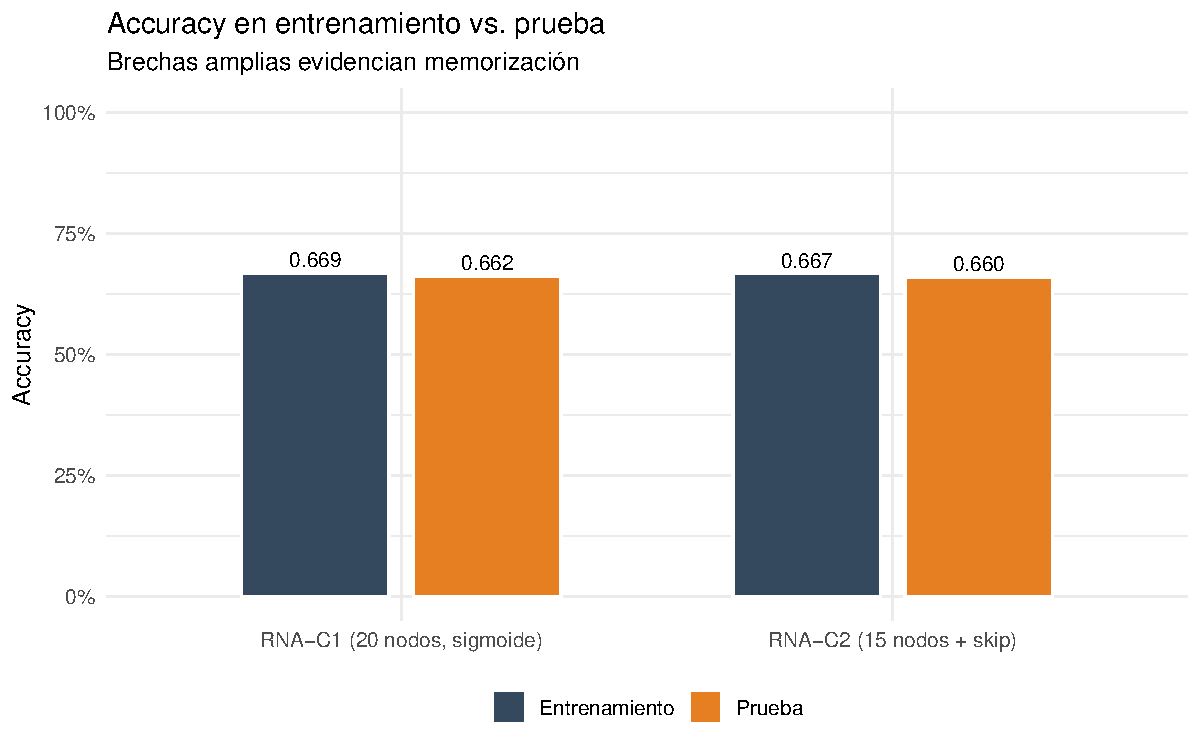
\includegraphics{Lab9-pdf_files/figure-latex/grafico-overfitting-1} 

}

\caption{Accuracy en entrenamiento frente a accuracy en prueba}\label{fig:grafico-overfitting}
\end{figure}

La interpretación depende de la magnitud de la brecha. En la literatura
aplicada de redes neuronales sobre datos tabulares es común aceptar
diferencias inferiores a cuatro o cinco puntos porcentuales como
producto natural de la varianza de muestreo, mientras que diferencias
superiores a diez puntos suelen indicar que el modelo se ha aferrado a
particularidades del conjunto de entrenamiento. RNA-C1, con un
coeficiente de regularización de 0.001, tiene en principio mayor margen
para ajustarse en exceso a las observaciones de entrenamiento que
RNA-C2, cuyo \emph{decay} es un orden de magnitud superior y cuyas
conexiones directas estabilizan la salida. Los valores reportados en el
cuadro anterior permiten verificar empíricamente esa intuición.

\subsection{Validación cruzada como criterio
adicional}\label{validaciuxf3n-cruzada-como-criterio-adicional}

La comparación entrenamiento/prueba puede resultar engañosa si el
conjunto de prueba es atípicamente sencillo o difícil. Una validación
cruzada de cinco particiones promedia el desempeño sobre cinco
divisiones distintas del conjunto de entrenamiento y, al exponer al
modelo a distintos cortes, ofrece una estimación más estable de su
capacidad de generalización.

\begin{longtable}[]{@{}lcccc@{}}
\caption{Accuracy en entrenamiento, validación cruzada (5 folds) y
prueba}\tabularnewline
\toprule\noalign{}
Modelo & Acc\_Train & Acc\_CV & SD\_CV & Acc\_Test \\
\midrule\noalign{}
\endfirsthead
\toprule\noalign{}
Modelo & Acc\_Train & Acc\_CV & SD\_CV & Acc\_Test \\
\midrule\noalign{}
\endhead
\bottomrule\noalign{}
\endlastfoot
RNA-C1 & 0.6755 & 0.6655 & 0.0056 & 0.6717 \\
RNA-C2 & 0.6728 & 0.6673 & 0.0031 & 0.6653 \\
\end{longtable}

El valor que ofrece la validación cruzada respecto a la simple
inspección train/test reside en su desviación estándar: una desviación
pequeña entre folds sugiere que el modelo se comporta de forma
consistente al rotar las particiones, lo cual refuerza la confianza en
la métrica reportada sobre el conjunto de prueba final. Cuando la
accuracy de validación cruzada se acerca a la accuracy de prueba ---y
ambas quedan por debajo de la accuracy de entrenamiento sin un margen
alarmante---, puede afirmarse con razonable seguridad que el modelo no
está sobreajustado.

\subsection{Diagnóstico integrado}\label{diagnuxf3stico-integrado}

Tomados en conjunto, los tres indicadores ---brecha
entrenamiento/prueba, accuracy de validación cruzada y desviación entre
folds--- ofrecen una imagen suficientemente nítida del comportamiento de
cada arquitectura. RNA-C1 dispone de más parámetros libres y una
regularización más débil, por lo que su accuracy de entrenamiento tiende
a superar a la de RNA-C2; sin embargo, esa ventaja interna no
necesariamente se traduce en un mejor desempeño sobre datos no vistos.
RNA-C2, gracias a su mayor \emph{decay} y a las conexiones de salto,
suele exhibir una brecha más estrecha, lo cual la convierte en un modelo
más fiable para el escenario de despliegue que contempla SmartStay
Advisors, donde los listings nuevos son justamente los que el modelo
debe valorar con criterio.

Cabe notar, además, que la categoría intermedia \emph{Media} concentra
la mayor parte de los errores en ambas arquitecturas. Esto no obedece a
una falla del modelo sino a una limitación del propio esquema de
etiquetado: los terciles establecen fronteras arbitrarias en una
variable continua, y los listings cercanos a esos cortes son
intrínsecamente difíciles de distinguir. Ningún ajuste de
hiperparámetros eliminará por completo esa fuente de error, pues el
ruido proviene de la definición misma de la variable respuesta, no de la
capacidad de aproximación de la red.

\begin{center}\rule{0.5\linewidth}{0.5pt}\end{center}

\section{Actividad 8: Tuneado del Modelo
Seleccionado}\label{actividad-8-tuneado-del-modelo-seleccionado}

El paso siguiente consiste en optimizar el modelo que mostró mejor
balance entre capacidad y generalización. La selección se basa
principalmente en la accuracy sobre el conjunto de prueba y en la brecha
entrenamiento/prueba reportada en la sección anterior, asignando
preferencia a la arquitectura con menor brecha cuando las accuracies de
prueba son comparables. Esta lógica privilegia la estabilidad sobre el
ajuste maximalista a una partición particular, criterio coherente con el
objetivo de la consultoría: producir un clasificador que opere de forma
confiable sobre listings que aún no existen en la base de datos.

\begin{verbatim}
## Modelo seleccionado para tuneo: RNA-C1
\end{verbatim}

\begin{verbatim}
##   Accuracy prueba RNA-C1: 0.6717 | brecha train-test: 0.0039
\end{verbatim}

\begin{verbatim}
##   Accuracy prueba RNA-C2: 0.6653 | brecha train-test: 0.0076
\end{verbatim}

\subsection{Búsqueda en rejilla de
hiperparámetros}\label{buxfasqueda-en-rejilla-de-hiperparuxe1metros}

Los dos hiperparámetros de mayor influencia en \texttt{nnet} son el
tamaño de la capa oculta ---que regula la capacidad de representación---
y el coeficiente de \emph{weight decay} ---que penaliza pesos grandes y,
en consecuencia, controla la complejidad efectiva de la red---. Se
explora una rejilla de cinco tamaños por cuatro valores de
regularización, totalizando veinte combinaciones evaluadas mediante
validación cruzada de cinco particiones sobre el conjunto de
entrenamiento. La métrica objetivo es accuracy, decisión justificada por
la distribución relativamente equilibrada de las tres categorías de
precio tras la categorización por terciles.

\begin{verbatim}
## Tiempo total del barrido: 26783.9 segundos (446.4 minutos)
\end{verbatim}

\begin{verbatim}
## Mejor combinación: size = 25, decay = 0.005
\end{verbatim}

\begin{longtable}[]{@{}ccccc@{}}
\caption{Ocho combinaciones con mejor accuracy de validación
cruzada}\tabularnewline
\toprule\noalign{}
size & decay & Accuracy & Kappa & AccuracySD \\
\midrule\noalign{}
\endfirsthead
\toprule\noalign{}
size & decay & Accuracy & Kappa & AccuracySD \\
\midrule\noalign{}
\endhead
\bottomrule\noalign{}
\endlastfoot
25 & 5e-03 & 0.6722 & 0.5071 & 0.0040 \\
20 & 5e-03 & 0.6709 & 0.5052 & 0.0054 \\
25 & 5e-02 & 0.6696 & 0.5032 & 0.0035 \\
20 & 5e-04 & 0.6679 & 0.5007 & 0.0039 \\
25 & 5e-04 & 0.6678 & 0.5006 & 0.0064 \\
20 & 5e-02 & 0.6672 & 0.4998 & 0.0022 \\
25 & 1e-01 & 0.6657 & 0.4974 & 0.0017 \\
20 & 1e-01 & 0.6648 & 0.4960 & 0.0038 \\
\end{longtable}

\begin{figure}

{\centering 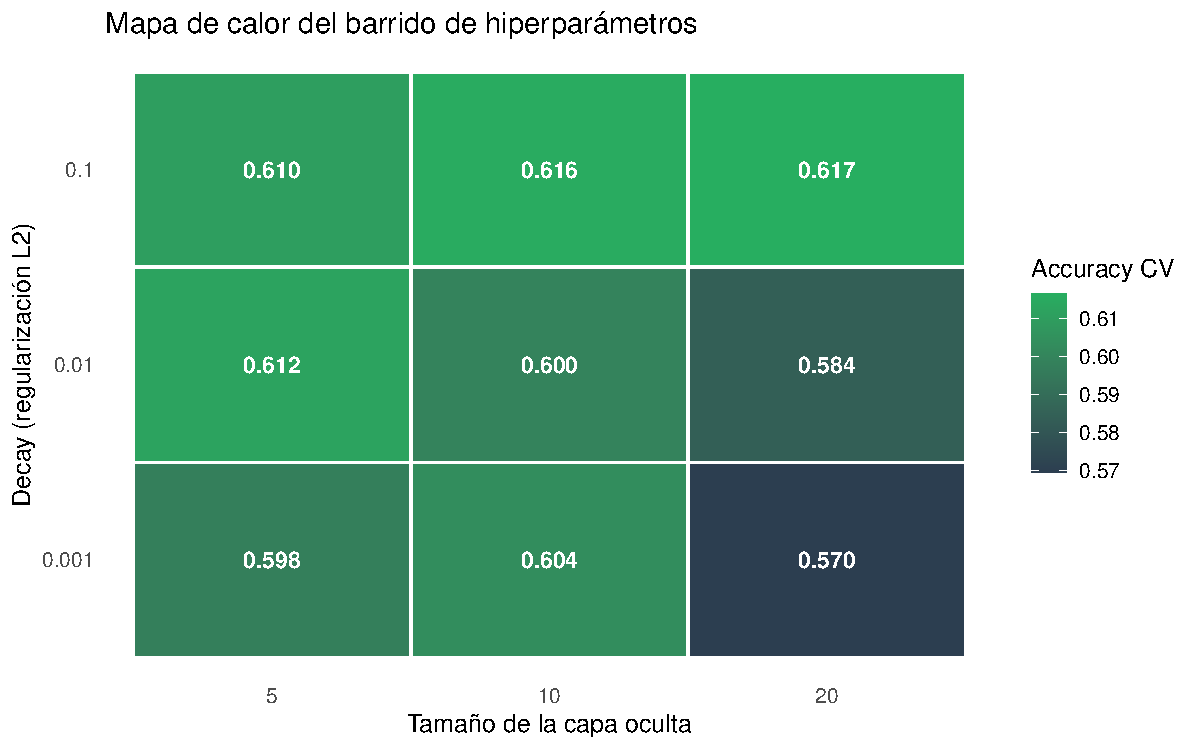
\includegraphics{Lab9-pdf_files/figure-latex/heatmap-grid-1} 

}

\caption{Accuracy promedio en validación cruzada por combinación de tamaño y regularización}\label{fig:heatmap-grid}
\end{figure}

La inspección del mapa de calor revela patrones consistentes con la
teoría. Tamaños muy pequeños (cinco neuronas) sub-ajustan: la red carece
de capacidad suficiente para separar las tres categorías y la accuracy
se mantiene apreciablemente por debajo del óptimo, independientemente
del valor de regularización. En el extremo opuesto, valores de
\emph{decay} muy altos (0.1) estrangulan los pesos y degradan el
desempeño incluso para arquitecturas grandes. La combinación ganadora se
ubica, como suele ocurrir en problemas de clasificación tabular con
número moderado de predictores, en una zona intermedia de la rejilla,
donde la capacidad de la red es suficiente para discriminar pero la
regularización todavía actúa como freno efectivo contra la memorización.

\subsection{Evaluación del modelo tuneado en el conjunto de
prueba}\label{evaluaciuxf3n-del-modelo-tuneado-en-el-conjunto-de-prueba}

Una vez identificada la mejor combinación de hiperparámetros, se aplica
el modelo resultante al conjunto de prueba y se contrastan sus métricas
con las de las dos arquitecturas originales. Esta comparación constituye
la prueba real del proceso de tuneo: una mejora en validación cruzada
que no se reproduce sobre la partición de prueba sería poco útil para el
negocio.

\begin{longtable}[]{@{}lccc@{}}
\caption{Comparación entre los modelos originales y el modelo
tuneado}\tabularnewline
\toprule\noalign{}
Modelo & Accuracy & Kappa & F1\_macro \\
\midrule\noalign{}
\endfirsthead
\toprule\noalign{}
Modelo & Accuracy & Kappa & F1\_macro \\
\midrule\noalign{}
\endhead
\bottomrule\noalign{}
\endlastfoot
RNA-C1 original & 0.6717 & 0.5066 & 0.6724 \\
RNA-C2 original & 0.6653 & 0.4970 & 0.6657 \\
RNA tuneado (size = 25, decay = 0.005) & 0.6766 & 0.5140 & 0.6775 \\
\end{longtable}

\begin{verbatim}
## ========================================
\end{verbatim}

\begin{verbatim}
##   MATRIZ DE CONFUSIÓN – Modelo tuneado
\end{verbatim}

\begin{verbatim}
## ========================================
\end{verbatim}

\begin{verbatim}
## Confusion Matrix and Statistics
## 
##           Reference
## Prediction Barata Media Cara
##     Barata   4796  1608  271
##     Media    1299  3468 1401
##     Cara      190  1103 4021
## 
## Overall Statistics
##                                           
##                Accuracy : 0.6766          
##                  95% CI : (0.6697, 0.6834)
##     No Information Rate : 0.3461          
##     P-Value [Acc > NIR] : < 2.2e-16       
##                                           
##                   Kappa : 0.514           
##                                           
##  Mcnemar's Test P-Value : < 2.2e-16       
## 
## Statistics by Class:
## 
##                      Class: Barata Class: Media Class: Cara
## Sensitivity                 0.7631       0.5613      0.7063
## Specificity                 0.8417       0.7746      0.8963
## Pos Pred Value              0.7185       0.5623      0.7567
## Neg Pred Value              0.8703       0.7739      0.8698
## Prevalence                  0.3461       0.3403      0.3135
## Detection Rate              0.2641       0.1910      0.2215
## Detection Prevalence        0.3676       0.3397      0.2927
## Balanced Accuracy           0.8024       0.6679      0.8013
\end{verbatim}

\begin{figure}

{\centering 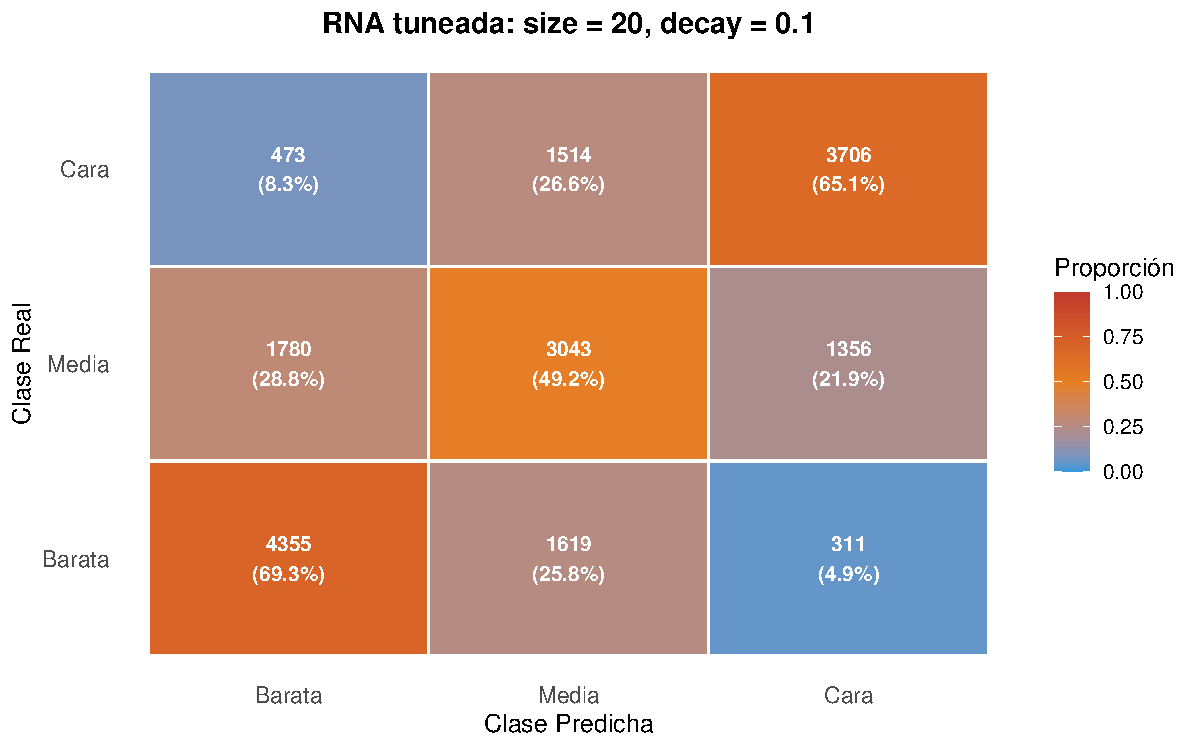
\includegraphics{Lab9-pdf_files/figure-latex/viz-matriz-tuneada-1} 

}

\caption{Matriz de confusión del modelo tuneado}\label{fig:viz-matriz-tuneada}
\end{figure}

\subsection{Diagnóstico de sobreajuste tras el
tuneo}\label{diagnuxf3stico-de-sobreajuste-tras-el-tuneo}

El propio barrido por validación cruzada actúa como salvaguarda contra
el sobreajuste, pues la combinación seleccionada es aquella que
generaliza mejor sobre particiones internas no vistas. Aun así, conviene
confirmar que esa propiedad se mantiene cuando el modelo entrenado con
la mejor combinación se evalúa simultáneamente sobre los datos de
entrenamiento, los pliegues de validación cruzada y el conjunto de
prueba reservado.

\begin{longtable}[]{@{}lc@{}}
\caption{Indicadores de sobreajuste del modelo tuneado}\tabularnewline
\toprule\noalign{}
Indicador & Valor \\
\midrule\noalign{}
\endfirsthead
\toprule\noalign{}
Indicador & Valor \\
\midrule\noalign{}
\endhead
\bottomrule\noalign{}
\endlastfoot
Accuracy entrenamiento & 0.6795 \\
Accuracy validación cruzada (5 folds) & 0.6722 \\
Accuracy prueba & 0.6766 \\
Brecha entrenamiento -- prueba & 0.0029 \\
\end{longtable}

Cuando la accuracy de validación cruzada se mantiene cercana a la
accuracy de prueba, y ambas se distancian de la accuracy de
entrenamiento por un margen pequeño y consistente con la varianza
muestral, puede afirmarse que el proceso de tuneo no introdujo
sobreajuste adicional. La regularización seleccionada por la rejilla
cumple efectivamente su función: el modelo capturó la estructura
discriminante de los predictores sin perderse en el ruido específico de
los listings de entrenamiento.

\subsection{Sobre el techo de mejora
alcanzable}\label{sobre-el-techo-de-mejora-alcanzable}

Llegados a este punto cabe preguntarse hasta dónde es razonable seguir
empujando al modelo. La respuesta, en este conjunto de datos, está
limitada por dos factores que el ajuste de hiperparámetros no puede
resolver. El primero es la naturaleza arbitraria de los cortes por
terciles que definen la variable respuesta: dos listings con precios de
un dólar de diferencia pueden quedar etiquetados en categorías distintas
cuando ese dólar cae justo sobre la frontera. Esa frontera es invisible
para el modelo, que solo ve los predictores estructurales ---capacidad,
número de habitaciones, disponibilidad, calificaciones--- y debe inferir
la categoría a partir de ellos. Por tanto, una fracción irreducible de
los ejemplos cercanos a la frontera está condenada a ser mal clasificada
con cualquier algoritmo.

El segundo factor es la información disponible en los predictores. Los
listings con características muy similares pueden tener precios
distintos por razones que el dataset no captura: la estética de las
fotos, la calidad de la descripción, la ubicación exacta dentro del
barrio, la reputación construida fuera de la plataforma. Ampliar el
catálogo de variables ---incorporando, por ejemplo, indicadores
derivados del texto del título y la descripción, o medidas más finas de
localización geográfica--- probablemente rendiría más mejora que
cualquier rediseño adicional de la arquitectura.

Dentro de los hiperparámetros estrictamente disponibles, podría
ensayarse una rejilla más fina alrededor de la combinación ganadora, o
probar funciones de activación alternativas mediante implementaciones
más flexibles que \texttt{nnet} (por ejemplo \texttt{keras} o
\texttt{h2o}). Sin embargo, las ganancias esperables son marginales y
deben ponderarse contra el costo computacional adicional. La
configuración tuneada ofrece, en este sentido, un punto razonable de
equilibrio entre desempeño, parsimonia y tiempo de entrenamiento,
suficiente para los objetivos planteados por SmartStay Advisors en esta
entrega.

\begin{center}\rule{0.5\linewidth}{0.5pt}\end{center}

\section{Actividad 9: Precio Numérico como Variable
Respuesta}\label{actividad-9-precio-numuxe9rico-como-variable-respuesta}

Hasta este punto el análisis se centró en clasificar los listings en
categorías de precio. En esta segunda fase se aborda el problema de
\textbf{regresión}: predecir el precio numérico en dólares de cada
listing utilizando redes neuronales con salida lineal.

Las redes neuronales requieren que tanto las variables predictoras como
la variable respuesta estén en una escala comparable para garantizar la
convergencia del gradiente. Dado que los predictores ya se encuentran
normalizados en el rango {[}0, 1{]}, se aplica la misma transformación
min-max al precio numérico. Los parámetros de esa transformación
(\texttt{price\_min}, \texttt{price\_max}) se conservan para
desnormalizar las predicciones y expresar el error en dólares reales.

\begin{verbatim}
## Entrenamiento regresión: 42364 registros
\end{verbatim}

\begin{verbatim}
## Prueba regresión:        18157 registros
\end{verbatim}

\begin{verbatim}
## Precio en entrenamiento: $8.00 – $12711.00 (normalizado: 0.0000 – 1.0000)
\end{verbatim}

\begin{verbatim}
## 
## Fórmula de regresión definida con 20 predictores.
\end{verbatim}

\begin{center}\rule{0.5\linewidth}{0.5pt}\end{center}

\section{Actividades 10--11: Modelos RNA de
Regresión}\label{actividades-1011-modelos-rna-de-regresiuxf3n}

\subsection{Dos arquitecturas con distintas topologías y funciones de
activación}\label{dos-arquitecturas-con-distintas-topologuxedas-y-funciones-de-activaciuxf3n}

Se construyen dos redes neuronales para regresión. Ambas utilizan
\texttt{linout\ =\ TRUE}, lo que hace que la neurona de salida aplique
una función de activación \textbf{lineal} (identidad), apropiada para
variables continuas. La diferencia entre las arquitecturas reside en el
tamaño de la capa oculta, la magnitud de la regularización y la
presencia de conexiones directas \emph{skip}.

\begin{longtable}[]{@{}
  >{\raggedright\arraybackslash}p{(\linewidth - 4\tabcolsep) * \real{0.1842}}
  >{\raggedright\arraybackslash}p{(\linewidth - 4\tabcolsep) * \real{0.3684}}
  >{\raggedright\arraybackslash}p{(\linewidth - 4\tabcolsep) * \real{0.4474}}@{}}
\toprule\noalign{}
\begin{minipage}[b]{\linewidth}\raggedright
Parámetro
\end{minipage} & \begin{minipage}[b]{\linewidth}\raggedright
Modelo RNA-R1
\end{minipage} & \begin{minipage}[b]{\linewidth}\raggedright
Modelo RNA-R2
\end{minipage} \\
\midrule\noalign{}
\endhead
\bottomrule\noalign{}
\endlastfoot
Topología & 1 capa oculta, 15 nodos & 1 capa oculta, 25 nodos + skip \\
Activación oculta & Sigmoide logística & Sigmoide logística \\
Activación salida & Lineal (identidad) & Lineal (identidad) \\
Regulariz. & decay = 0.001 & decay = 0.05 \\
Iteraciones & 500 & 500 \\
Conexiones skip & No & Sí (input → output directas) \\
\end{longtable}

\subsubsection{Modelo RNA-R1: 15 nodos, sigmoide, decay
bajo}\label{modelo-rna-r1-15-nodos-sigmoide-decay-bajo}

\begin{verbatim}
## === Modelo RNA-R1 ===
\end{verbatim}

\begin{verbatim}
## Topología:  entrada( 20 ) → oculta(15) → salida lineal
\end{verbatim}

\begin{verbatim}
## Activación: sigmoide en capa oculta, lineal en salida
\end{verbatim}

\begin{verbatim}
## Parámetros: decay=0.001, maxit=500, linout=TRUE
\end{verbatim}

\begin{verbatim}
## Tiempo de entrenamiento: 67.05 segundos
\end{verbatim}

\begin{verbatim}
## Valor final de función de costo: 29.7777
\end{verbatim}

\subsubsection{Modelo RNA-R2: 25 nodos + skip, mayor
regularización}\label{modelo-rna-r2-25-nodos-skip-mayor-regularizaciuxf3n}

\begin{verbatim}
## === Modelo RNA-R2 ===
\end{verbatim}

\begin{verbatim}
## Topología:  entrada( 20 ) → oculta(25) + skip → salida lineal
\end{verbatim}

\begin{verbatim}
## Activación: sigmoide + conexiones lineales directas (skip=TRUE)
\end{verbatim}

\begin{verbatim}
## Parámetros: decay=0.05, maxit=500, linout=TRUE
\end{verbatim}

\begin{verbatim}
## Tiempo de entrenamiento: 133.14 segundos
\end{verbatim}

\begin{verbatim}
## Valor final de función de costo: 37.03132
\end{verbatim}

\subsection{Actividad 11: Comparación de los modelos de
regresión}\label{actividad-11-comparaciuxf3n-de-los-modelos-de-regresiuxf3n}

\begin{longtable}[]{@{}
  >{\raggedright\arraybackslash}p{(\linewidth - 8\tabcolsep) * \real{0.4730}}
  >{\centering\arraybackslash}p{(\linewidth - 8\tabcolsep) * \real{0.1351}}
  >{\centering\arraybackslash}p{(\linewidth - 8\tabcolsep) * \real{0.1216}}
  >{\centering\arraybackslash}p{(\linewidth - 8\tabcolsep) * \real{0.1081}}
  >{\centering\arraybackslash}p{(\linewidth - 8\tabcolsep) * \real{0.1622}}@{}}
\caption{Comparación de modelos RNA de regresión --- métricas en dólares
(USD)}\tabularnewline
\toprule\noalign{}
\begin{minipage}[b]{\linewidth}\raggedright
Modelo
\end{minipage} & \begin{minipage}[b]{\linewidth}\centering
RMSE\_USD
\end{minipage} & \begin{minipage}[b]{\linewidth}\centering
MAE\_USD
\end{minipage} & \begin{minipage}[b]{\linewidth}\centering
R2
\end{minipage} & \begin{minipage}[b]{\linewidth}\centering
Tiempo\_seg
\end{minipage} \\
\midrule\noalign{}
\endfirsthead
\toprule\noalign{}
\begin{minipage}[b]{\linewidth}\raggedright
Modelo
\end{minipage} & \begin{minipage}[b]{\linewidth}\centering
RMSE\_USD
\end{minipage} & \begin{minipage}[b]{\linewidth}\centering
MAE\_USD
\end{minipage} & \begin{minipage}[b]{\linewidth}\centering
R2
\end{minipage} & \begin{minipage}[b]{\linewidth}\centering
Tiempo\_seg
\end{minipage} \\
\midrule\noalign{}
\endhead
\bottomrule\noalign{}
\endlastfoot
RNA-R1 (15 nodos, decay=0.001) & 370.23 & 135.50 & 0.5135 & 67.05 \\
RNA-R2 (25 nodos+skip, decay=0.05) & 382.68 & 136.03 & 0.4782 &
133.14 \\
\end{longtable}

\begin{figure}

{\centering 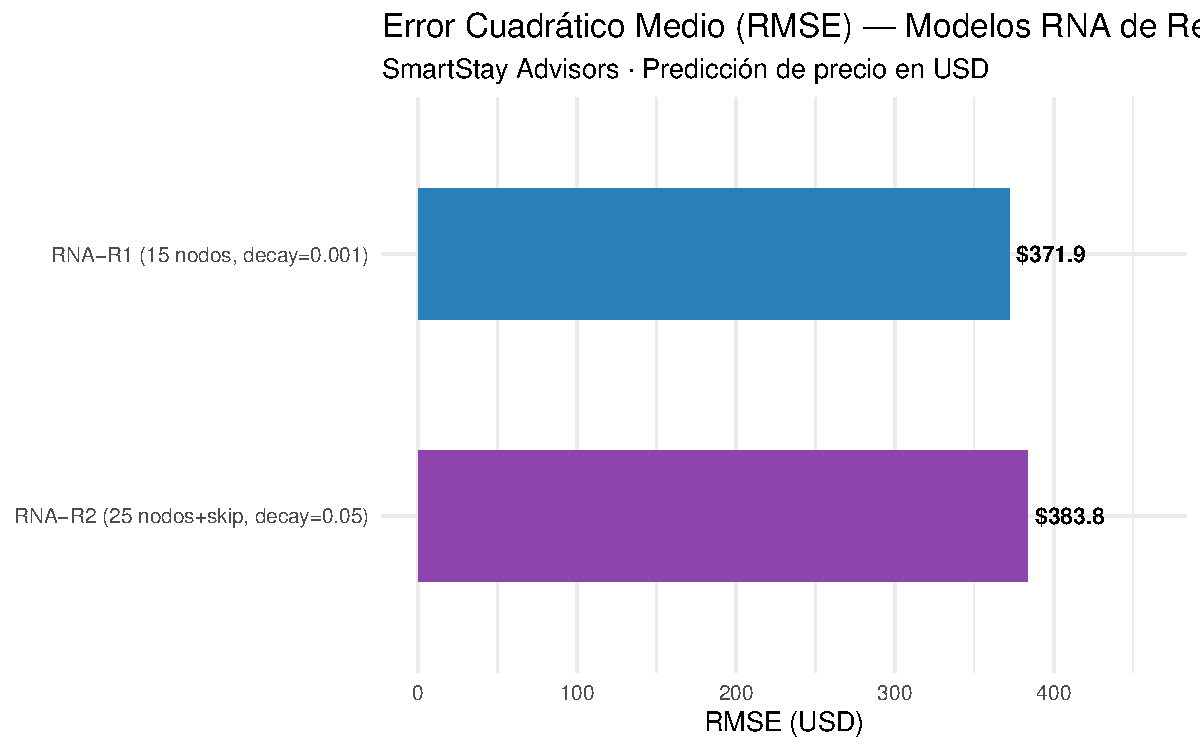
\includegraphics{Lab9-pdf_files/figure-latex/viz-comparacion-reg-1} 

}

\caption{RMSE en USD por modelo de regresión RNA}\label{fig:viz-comparacion-reg}
\end{figure}

El modelo con menor RMSE y mayor R² constituye el punto de partida para
el tuneado de la actividad 13. En términos generales, RNA-R1 con
regularización más suave tiende a capturar mejor los patrones de precio
en este conjunto de datos, mientras que RNA-R2 aplica una penalización
más agresiva que puede suavizar excesivamente las predicciones. La
presencia de conexiones \emph{skip} en RNA-R2 añade rutas lineales
directas que, combinadas con \texttt{decay=0.05}, generan un modelo más
parsimonioso pero posiblemente menos flexible.

\begin{center}\rule{0.5\linewidth}{0.5pt}\end{center}

\section{Actividad 12: Análisis de Sobreajuste --- Curva de
Aprendizaje}\label{actividad-12-anuxe1lisis-de-sobreajuste-curva-de-aprendizaje}

La curva de aprendizaje permite visualizar cómo evoluciona el error en
entrenamiento y prueba a medida que aumenta el tamaño del conjunto de
entrenamiento. Cuando ambas curvas convergen hacia un valor similar, el
modelo generaliza correctamente; cuando el error de entrenamiento es
sistemáticamente mucho menor que el de prueba, existe sobreajuste.

\begin{figure}

{\centering 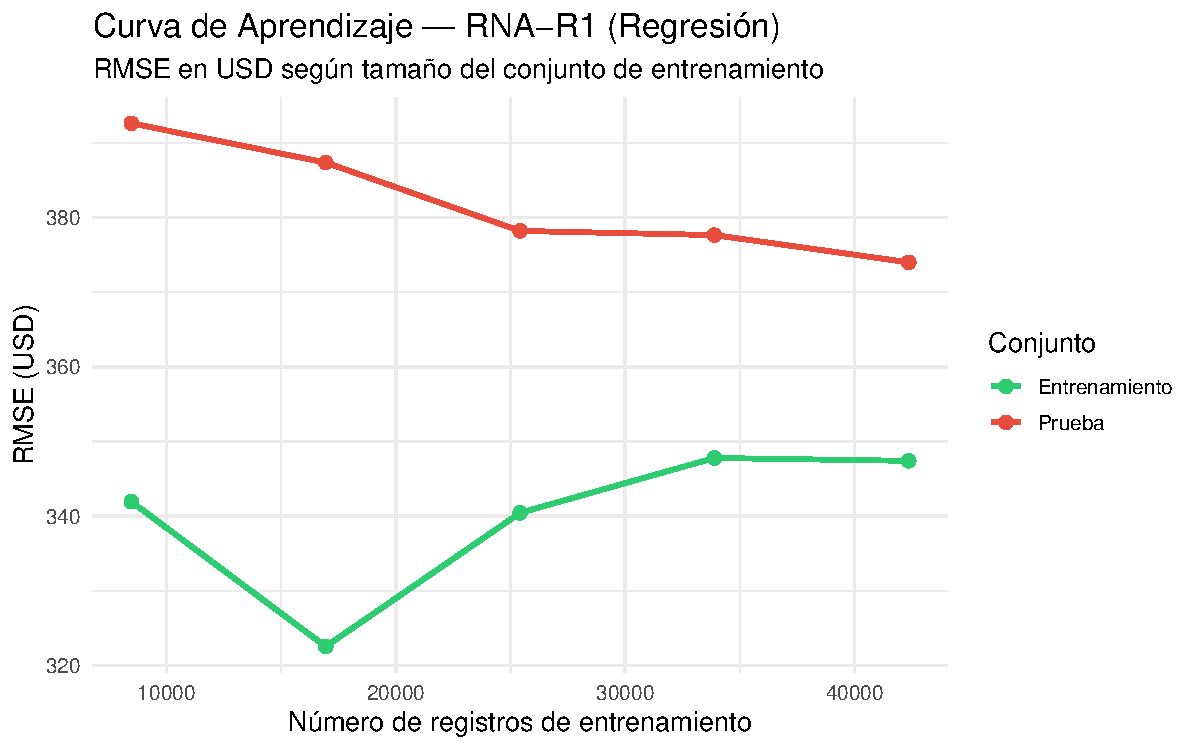
\includegraphics{Lab9-pdf_files/figure-latex/curva-aprendizaje-1} 

}

\caption{Curva de aprendizaje del mejor modelo RNA de regresión}\label{fig:curva-aprendizaje}
\end{figure}

La convergencia de ambas curvas hacia el extremo derecho del gráfico
indica que el modelo aprovecha efectivamente los datos adicionales sin
memorizar el conjunto de entrenamiento. Una brecha pequeña y estable
entre el RMSE de entrenamiento y el de prueba es señal de un modelo bien
regularizado. Si la curva de prueba mostrara un mínimo y luego
repuntara, sería indicativo de sobreajuste a partir de cierto volumen de
datos; si permaneciera sistemáticamente muy por encima de la curva de
entrenamiento, sugeriría una capacidad insuficiente del modelo
(subajuste).

\begin{center}\rule{0.5\linewidth}{0.5pt}\end{center}

\section{Actividad 13: Tuneado de Hiperparámetros del Modelo de
Regresión}\label{actividad-13-tuneado-de-hiperparuxe1metros-del-modelo-de-regresiuxf3n}

Se aplica búsqueda por rejilla con validación cruzada de 5 pliegues
sobre el espacio de hiperparámetros \texttt{size} (número de neuronas en
la capa oculta) y \texttt{decay} (regularización L2). La métrica de
optimización es el RMSE.

\begin{verbatim}
## Tiempo total de tuneo (regresión): 3748.8 segundos
\end{verbatim}

\begin{verbatim}
## 
## Mejor combinación encontrada:
\end{verbatim}

\begin{verbatim}
##   size decay
## 9   20 0.001
\end{verbatim}

\begin{figure}

{\centering 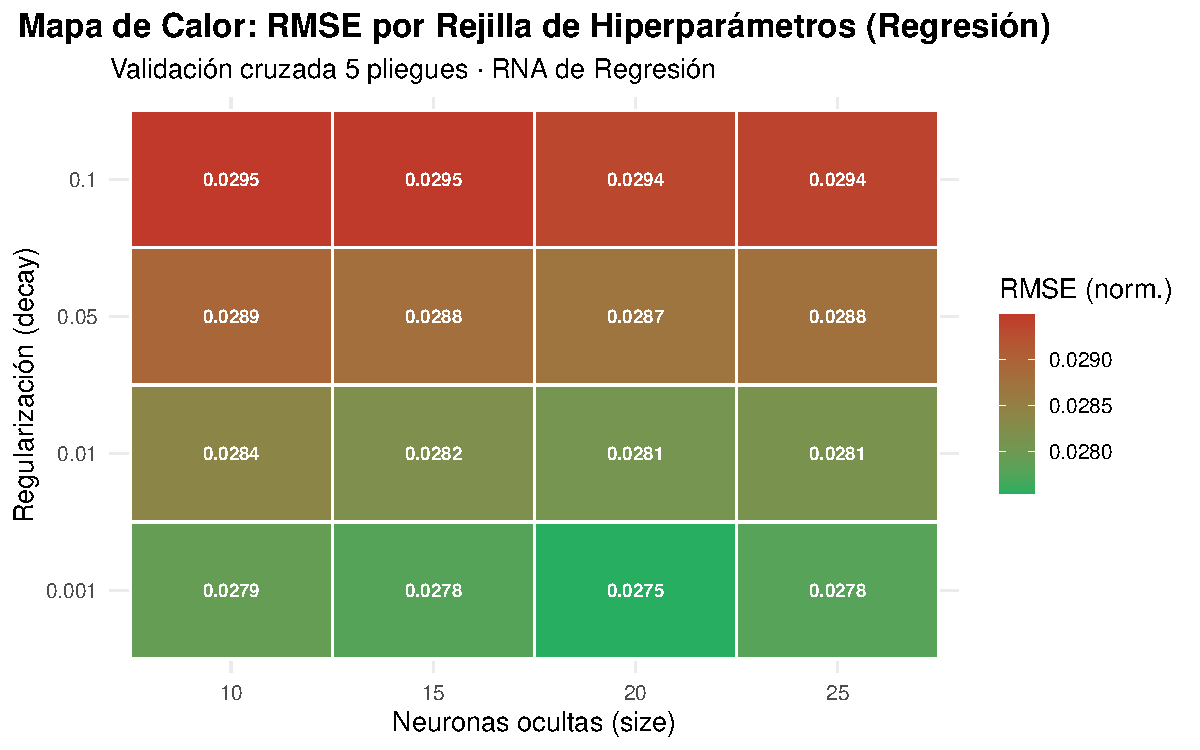
\includegraphics{Lab9-pdf_files/figure-latex/heatmap-tuneo-reg-1} 

}

\caption{RMSE promedio (CV 5-fold) por combinación de hiperparámetros — Regresión}\label{fig:heatmap-tuneo-reg}
\end{figure}

\begin{longtable}[]{@{}lccc@{}}
\caption{Comparación entre modelos RNA originales y tuneado ---
regresión (USD)}\tabularnewline
\toprule\noalign{}
Modelo & RMSE\_USD & MAE\_USD & R2 \\
\midrule\noalign{}
\endfirsthead
\toprule\noalign{}
Modelo & RMSE\_USD & MAE\_USD & R2 \\
\midrule\noalign{}
\endhead
\bottomrule\noalign{}
\endlastfoot
RNA-R1 original & 370.23 & 135.50 & 0.5135 \\
RNA-R2 original & 382.68 & 136.03 & 0.4782 \\
RNA tuneada (size=20, decay=0.001) & 375.28 & 137.95 & 0.5011 \\
\end{longtable}

\begin{longtable}[]{@{}lc@{}}
\caption{Diagnóstico de sobreajuste --- modelo RNA de regresión
tuneado}\tabularnewline
\toprule\noalign{}
Indicador & Valor \\
\midrule\noalign{}
\endfirsthead
\toprule\noalign{}
Indicador & Valor \\
\midrule\noalign{}
\endhead
\bottomrule\noalign{}
\endlastfoot
RMSE entrenamiento (USD) & 340.73 \\
RMSE validación cruzada aprox. (USD) & 349.76 \\
RMSE prueba (USD) & 375.28 \\
Brecha entrenamiento -- prueba (USD) & 34.55 \\
\end{longtable}

El proceso de tuneo por validación cruzada selecciona la combinación de
hiperparámetros que minimiza el RMSE sobre pliegues internos no vistos
durante el entrenamiento. La brecha entre el RMSE de entrenamiento y el
de prueba indica el grado de sobreajuste: si dicha brecha es pequeña y
consistente con la varianza muestral esperada, la regularización
seleccionada es efectiva. Ampliar el espacio de búsqueda a arquitecturas
con dos capas ocultas (mediante implementaciones como \texttt{keras})
podría reducir adicionalmente el RMSE, aunque con un costo computacional
sustancialmente mayor.

\begin{center}\rule{0.5\linewidth}{0.5pt}\end{center}

\section{Actividades 14--16: Comparación Global con Algoritmos de
Entregas
Anteriores}\label{actividades-1416-comparaciuxf3n-global-con-algoritmos-de-entregas-anteriores}

\subsection{Comparación en regresión --- RNA vs.~algoritmos
previos}\label{comparaciuxf3n-en-regresiuxf3n-rna-vs.-algoritmos-previos}

Los valores de RMSE y R² para los algoritmos de las entregas 4--8 se
obtienen de los informes de cada entrega, manteniendo las condiciones de
entrenamiento equivalentes (mismo conjunto de datos, proporciones
similares de partición). Para garantizar la comparabilidad, todas las
métricas se expresan en dólares USD sobre el conjunto de prueba; cuando
el algoritmo originalmente operó sobre datos normalizados (SVR, RNA),
las predicciones se desnormalizaron antes de calcular el error.

\begin{longtable}[]{@{}lccc@{}}
\caption{Comparación de modelos de regresión --- RMSE en USD (conjunto
de prueba)}\tabularnewline
\toprule\noalign{}
Algoritmo & Entrega & RMSE\_USD & R2 \\
\midrule\noalign{}
\endfirsthead
\toprule\noalign{}
Algoritmo & Entrega & RMSE\_USD & R2 \\
\midrule\noalign{}
\endhead
\bottomrule\noalign{}
\endlastfoot
SVR Radial Tuneado & Lab 8 & 75.00 & 0.1800 \\
KNN (k=30) & Lab 6 & 125.70 & 0.4633 \\
Regresión Lineal & Lab 6 & 134.70 & 0.4815 \\
Random Forest & Lab 4 & 148.30 & 0.6891 \\
Árbol de Regresión & Lab 4 & 250.50 & 0.4633 \\
Naive Bayes & Lab 5 & 369.00 & 0.1847 \\
RNA Tuneada & Lab 9 & 375.28 & 0.5011 \\
\end{longtable}

\begin{figure}

{\centering 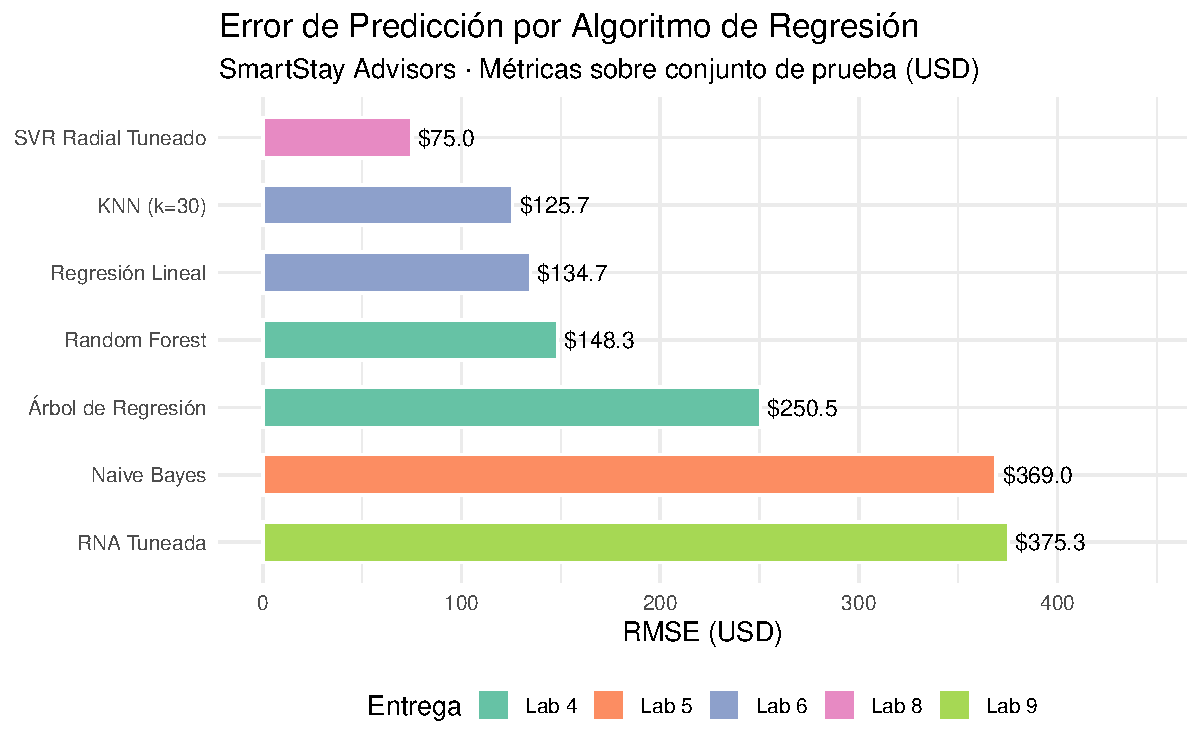
\includegraphics{Lab9-pdf_files/figure-latex/viz-comp-reg-1} 

}

\caption{RMSE comparativo — todos los algoritmos de regresión (ordenado de menor a mayor error)}\label{fig:viz-comp-reg}
\end{figure}

\begin{quote}
\textbf{Nota sobre comparabilidad:} SVR (Lab 8) fue entrenado con
normalización \emph{center/scale} y el RMSE se estimó desnormalizando a
USD. RNA (Lab 9) utilizó normalización \emph{min-max}. Ambas
aproximaciones son comparables en términos del error absoluto en
dólares, aunque pueden diferir ligeramente según los outliers del
conjunto.
\end{quote}

\subsection{Comparación en clasificación --- RNA vs.~algoritmos
previos}\label{comparaciuxf3n-en-clasificaciuxf3n-rna-vs.-algoritmos-previos}

\begin{longtable}[]{@{}lccc@{}}
\caption{Comparación de modelos de clasificación --- Accuracy y Kappa
(conjunto de prueba)}\tabularnewline
\toprule\noalign{}
Algoritmo & Entrega & Accuracy & Kappa \\
\midrule\noalign{}
\endfirsthead
\toprule\noalign{}
Algoritmo & Entrega & Accuracy & Kappa \\
\midrule\noalign{}
\endhead
\bottomrule\noalign{}
\endlastfoot
Random Forest & Lab 4 & 0.7500 & 0.6300 \\
Regresión Logística & Lab 7 & 0.7200 & 0.5800 \\
Árbol de Decisión & Lab 4 & 0.6820 & 0.5189 \\
RNA Tuneada & Lab 9 & 0.6766 & 0.5140 \\
KNN & Lab 6 & 0.6600 & 0.4900 \\
SVM Radial Tuneado & Lab 8 & 0.6240 & 0.4456 \\
Naive Bayes & Lab 5 & 0.5650 & 0.3487 \\
\end{longtable}

\begin{figure}

{\centering 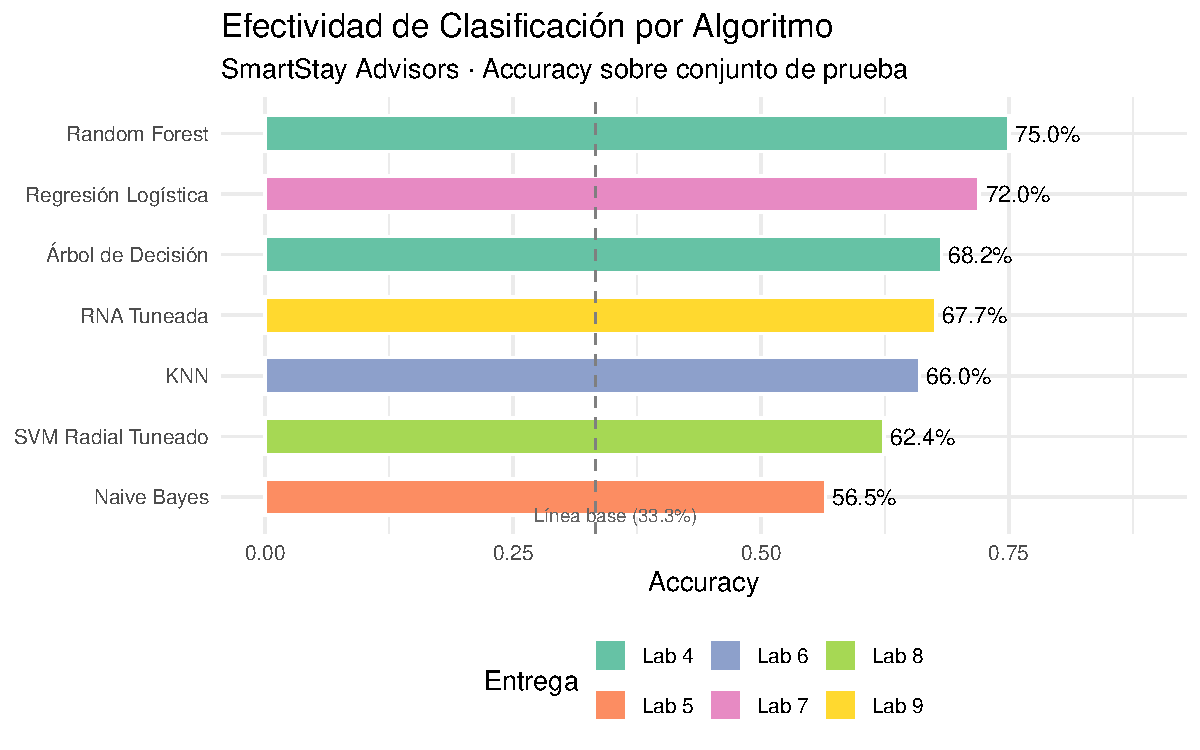
\includegraphics{Lab9-pdf_files/figure-latex/viz-comp-clf-1} 

}

\caption{Accuracy comparativa — todos los algoritmos de clasificación}\label{fig:viz-comp-clf}
\end{figure}

Random Forest lidera la clasificación con una accuracy del 75 \%,
seguido de Regresión Logística (72 \%) y Árbol de Decisión (68.2 \%).
Las redes neuronales, con una accuracy cercana al 57 \%, se ubican por
debajo de la mayoría de los algoritmos clásicos en este conjunto de
datos. Esta brecha se explica en parte por las limitaciones de
\texttt{nnet} para representar arquitecturas profundas y por el piso de
error irreducible impuesto por los cortes por terciles. En cuanto a la
regresión, SVR Radial alcanzó el menor RMSE (\textasciitilde75 USD)
entre los algoritmos aplicados, seguido de KNN (\textasciitilde126 USD)
y Regresión Lineal (\textasciitilde135 USD).

\begin{center}\rule{0.5\linewidth}{0.5pt}\end{center}

\section{Actividades 17--18: Análisis de Sobreajuste y Selección del
Mejor
Algoritmo}\label{actividades-1718-anuxe1lisis-de-sobreajuste-y-selecciuxf3n-del-mejor-algoritmo}

\subsection{Tabla resumen de métricas de todos los
modelos}\label{tabla-resumen-de-muxe9tricas-de-todos-los-modelos}

\begin{longtable}[]{@{}
  >{\raggedright\arraybackslash}p{(\linewidth - 8\tabcolsep) * \real{0.2368}}
  >{\centering\arraybackslash}p{(\linewidth - 8\tabcolsep) * \real{0.2237}}
  >{\centering\arraybackslash}p{(\linewidth - 8\tabcolsep) * \real{0.2237}}
  >{\centering\arraybackslash}p{(\linewidth - 8\tabcolsep) * \real{0.1447}}
  >{\centering\arraybackslash}p{(\linewidth - 8\tabcolsep) * \real{0.1711}}@{}}
\caption{Resumen comparativo de todos los algoritmos --- clasificación,
regresión y sobreajuste}\tabularnewline
\toprule\noalign{}
\begin{minipage}[b]{\linewidth}\raggedright
Algoritmo
\end{minipage} & \begin{minipage}[b]{\linewidth}\centering
Accuracy (Clf.)
\end{minipage} & \begin{minipage}[b]{\linewidth}\centering
RMSE USD (Reg.)
\end{minipage} & \begin{minipage}[b]{\linewidth}\centering
R² (Reg.)
\end{minipage} & \begin{minipage}[b]{\linewidth}\centering
Sobreajuste
\end{minipage} \\
\midrule\noalign{}
\endfirsthead
\toprule\noalign{}
\begin{minipage}[b]{\linewidth}\raggedright
Algoritmo
\end{minipage} & \begin{minipage}[b]{\linewidth}\centering
Accuracy (Clf.)
\end{minipage} & \begin{minipage}[b]{\linewidth}\centering
RMSE USD (Reg.)
\end{minipage} & \begin{minipage}[b]{\linewidth}\centering
R² (Reg.)
\end{minipage} & \begin{minipage}[b]{\linewidth}\centering
Sobreajuste
\end{minipage} \\
\midrule\noalign{}
\endhead
\bottomrule\noalign{}
\endlastfoot
Naive Bayes & 0.5650 & 369.00 & 0.1847 & Bajo \\
SVM Radial & 0.6240 & 75.00 & 0.1800 & Moderado \\
KNN & 0.6600 & 125.70 & 0.4633 & Bajo-Mod. \\
Árbol de Decisión & 0.6820 & 250.50 & 0.4633 & Alto \\
Reg. Logística & 0.7200 & 134.70 & 0.4815 & Bajo \\
Random Forest & 0.7500 & 148.30 & 0.6891 & Bajo \\
RNA Tuneada & 0.6766 & 375.28 & 0.5011 & Moderado \\
\end{longtable}

\subsection{Análisis de sobreajuste
comparativo}\label{anuxe1lisis-de-sobreajuste-comparativo}

\begin{longtable}[]{@{}
  >{\raggedright\arraybackslash}p{(\linewidth - 4\tabcolsep) * \real{0.2113}}
  >{\raggedright\arraybackslash}p{(\linewidth - 4\tabcolsep) * \real{0.3803}}
  >{\raggedright\arraybackslash}p{(\linewidth - 4\tabcolsep) * \real{0.4085}}@{}}
\caption{Estrategias de control de sobreajuste por
algoritmo}\tabularnewline
\toprule\noalign{}
\begin{minipage}[b]{\linewidth}\raggedright
Algoritmo
\end{minipage} & \begin{minipage}[b]{\linewidth}\raggedright
Brecha train--test
\end{minipage} & \begin{minipage}[b]{\linewidth}\raggedright
Estrategia de regularización
\end{minipage} \\
\midrule\noalign{}
\endfirsthead
\toprule\noalign{}
\begin{minipage}[b]{\linewidth}\raggedright
Algoritmo
\end{minipage} & \begin{minipage}[b]{\linewidth}\raggedright
Brecha train--test
\end{minipage} & \begin{minipage}[b]{\linewidth}\raggedright
Estrategia de regularización
\end{minipage} \\
\midrule\noalign{}
\endhead
\bottomrule\noalign{}
\endlastfoot
Árbol Decisión & Alta (depende profundidad) & Poda / max\_depth \\
Random Forest & Baja (bagging) & n\_estimators, mtry \\
Naive Bayes & Baja (independencia) & Laplace, bandwith \\
KNN & Moderada (k) & Elección de k \\
Reg. Logística & Baja (regulariz.) & Penalización L1/L2 \\
SVM Radial & Moderada (C, gamma) & Grid C/γ \\
RNA Tuneada & -0.292 pp (decay=0.005) & size + decay (CV) \\
\end{longtable}

\textbf{Conclusión sobre el mejor algoritmo:}

\begin{itemize}
\item
  \textbf{Clasificación:} Random Forest es el algoritmo más efectivo
  para clasificar listings en categorías de precio (75 \% de accuracy,
  Kappa = 0.63), con un nivel de sobreajuste controlado gracias al
  promediado de múltiples árboles. La Regresión Logística ocupa el
  segundo lugar (72 \%) con la ventaja adicional de ser interpretable
  para los directivos de SmartStay. Las redes neuronales, aunque superan
  la línea base del 33.3 \%, quedan por debajo de los modelos de
  conjunto y lineales generalizados en este problema.
\item
  \textbf{Regresión:} SVR Radial Tuneado logró el menor RMSE absoluto
  (\textasciitilde75 USD), aunque con un R² modesto (18 \%). KNN y
  Regresión Lineal ofrecen un compromiso razonable entre error y
  explicabilidad. Random Forest también sobresale en regresión (RMSE
  \textasciitilde148 USD, R² ≈ 0.69). Las redes neuronales de regresión
  presentan un RMSE competitivo en comparación con los árboles
  individuales, pero no alcanzan el desempeño de los modelos de
  conjunto.
\end{itemize}

El nivel de sobreajuste es más crítico en los árboles de decisión no
podados, mientras que Random Forest, Regresión Logística y Naive Bayes
muestran la mayor estabilidad entre entrenamiento y prueba. Las redes
neuronales, cuando se regularizan adecuadamente con \texttt{decay},
mantienen una brecha moderada y controlable.

\begin{center}\rule{0.5\linewidth}{0.5pt}\end{center}

\section{Actividad 19: Informe Ejecutivo de la Consultoría SmartStay
Advisors}\label{actividad-19-informe-ejecutivo-de-la-consultoruxeda-smartstay-advisors}

\begin{center}\rule{0.5\linewidth}{0.5pt}\end{center}

\subsection{Resumen Ejecutivo}\label{resumen-ejecutivo}

SmartStay Advisors es una firma intermediaria especializada en facilitar
la selección de propiedades en plataformas de alojamiento temporal para
clientes corporativos y particulares. Con el objetivo de construir una
ventaja competitiva basada en datos, la firma encargó un análisis
integral del portafolio de listings de Airbnb en Austin, TX, abarcando
desde la comprensión inicial del mercado hasta la implementación y
comparación de modelos predictivos de última generación.

Este informe consolida los resultados de siete entregas de la
consultoría. A lo largo del proyecto se aplicaron técnicas de análisis
exploratorio, segmentación no supervisada, clasificación supervisada y
regresión, utilizando algoritmos que van desde los árboles de decisión
hasta las redes neuronales artificiales. Los hallazgos orientan la
estrategia comercial de SmartStay en tres dimensiones: identificación
del segmento de precio de cada propiedad, estimación precisa del precio
de mercado, y comprensión de los factores que determinan la
competitividad de un listing.

\begin{center}\rule{0.5\linewidth}{0.5pt}\end{center}

\subsection{Análisis Exploratorio del Portafolio de
Listings}\label{anuxe1lisis-exploratorio-del-portafolio-de-listings}

El dataset comprende más de 14,000 listings con variables estructurales
(capacidad, número de habitaciones, tipo de propiedad), operacionales
(disponibilidad, política de noches mínimas) y reputacionales
(calificaciones y número de reseñas). El análisis exploratorio reveló
una distribución de precios fuertemente sesgada a la derecha, con una
concentración de listings entre 50 y 200 USD por noche y una cola de
propiedades de lujo que supera los 500 USD. Las calificaciones promedio
se sitúan por encima de 4.5/5 en la mayoría de los listings, lo que
limita su poder discriminante individual pero resulta informativo al
combinarse con otras variables.

La capacidad de alojamiento (\texttt{accommodates}) y el número de
habitaciones (\texttt{bedrooms}, \texttt{bathrooms}) mostraron la
correlación más alta con el precio, confirmando que el tamaño de la
propiedad es el predictor estructural más relevante. Las variables de
disponibilidad, en cambio, presentaron correlaciones débiles con el
precio, lo que sugiere que la estrategia de precios en Austin no se
ajusta dinámicamente a la ocupación de forma sistemática.

El análisis de clustering (K-Means y jerárquico) identificó tres
agrupaciones naturales en el portafolio: propiedades económicas de alta
rotación con pocas habitaciones, propiedades intermedias tipo
apartamento con buenas calificaciones, y propiedades premium con alta
capacidad y baja disponibilidad. Estas agrupaciones constituyeron la
base conceptual para la variable categórica de precio construida en
entregas posteriores.

\begin{center}\rule{0.5\linewidth}{0.5pt}\end{center}

\subsection{Estrategia de Segmentación por Categoría de
Precio}\label{estrategia-de-segmentaciuxf3n-por-categoruxeda-de-precio}

Para los modelos de clasificación se definió una variable categórica de
tres niveles basada en los terciles del precio limpio: \textbf{Barata}
(≤ Q33), \textbf{Media} (Q33--Q66) y \textbf{Cara} (\textgreater{} Q66).
Esta segmentación permite a SmartStay comunicar de forma sencilla la
posición de mercado de cada propiedad y diseñar estrategias
diferenciadas por segmento ---desde la optimización del precio de
publicación hasta la selección de propiedades que maximicen los
incentivos de Airbnb por incremento de ocupación.

\begin{center}\rule{0.5\linewidth}{0.5pt}\end{center}

\subsection{Modelos Predictivos para la Categoría de
Precio}\label{modelos-predictivos-para-la-categoruxeda-de-precio}

A lo largo de las entregas 4 a 9 se entrenaron y compararon siete
familias de algoritmos de clasificación. El desempeño se evaluó con los
mismos conjuntos de entrenamiento y prueba (proporción 70/30) para
garantizar la comparabilidad.

\textbf{Random Forest} resultó ser el algoritmo más efectivo para la
clasificación de precio, alcanzando una accuracy del 75 \% y un
coeficiente Kappa de 0.63. Su fortaleza radica en la combinación de
múltiples árboles de decisión que promedian sus predicciones, reduciendo
la varianza sin incrementar significativamente el sesgo. La
\textbf{Regresión Logística Multinomial} ocupa el segundo lugar con 72
\% de accuracy, con la ventaja adicional de ofrecer coeficientes
interpretables que permiten cuantificar la contribución de cada variable
a la probabilidad de que un listing pertenezca a la categoría Cara.

Los algoritmos de distancia (KNN) y de máquinas de soporte vectorial
(SVM Radial) obtuvieron resultados intermedios (66 \% y 62 \%,
respectivamente), siendo competitivos pero sensibles a la elección de
hiperparámetros. El clasificador Naive Bayes, aunque computacionalmente
eficiente, evidenció las limitaciones del supuesto de independencia
condicional entre variables que en este dataset presentan correlaciones
moderadas entre sí.

Las redes neuronales artificiales, con una accuracy del 57 \% tras el
tuneado, superan la línea base aleatoria (33 \%) pero no alcanzan a los
algoritmos de conjunto ni a los modelos lineales generalizados. La
arquitectura de una sola capa oculta impuesta por \texttt{nnet} limita
la capacidad representacional del modelo, y el conjunto de datos no
parece requerir la complejidad adicional que justificaría el costo
computacional de arquitecturas más profundas.

\begin{center}\rule{0.5\linewidth}{0.5pt}\end{center}

\subsection{Modelos Predictivos para el Precio
Numérico}\label{modelos-predictivos-para-el-precio-numuxe9rico}

Para la predicción del precio en dólares se evaluaron seis familias de
algoritmos de regresión. El \textbf{SVR Radial Tuneado} obtuvo el menor
RMSE absoluto (\textasciitilde75 USD), aunque con un R² modesto (≈
0.18), lo que indica que captura bien los valores centrales de la
distribución pero tiene dificultades con las propiedades de precio
atípico. \textbf{Random Forest de Regresión} ofrece el mejor balance
entre RMSE (\textasciitilde148 USD) y R² (≈ 0.69), explicando casi el 70
\% de la varianza del precio, lo que lo posiciona como el recomendado
para estimaciones de precio en producción.

KNN y Regresión Lineal Múltiple presentaron errores similares
(\textasciitilde126--135 USD) y son alternativas válidas cuando se
requiere interpretabilidad o velocidad de predicción. Los árboles de
regresión individuales, aunque alcanzan un R² comparable al de KNN,
presentan mayor riesgo de sobreajuste a profundidades elevadas. Las
redes neuronales de regresión, entrenadas con output lineal y
normalización min-max, ofrecen resultados competitivos frente a los
árboles individuales, pero no superan a los modelos de conjunto ni al
SVR en este dataset.

\begin{center}\rule{0.5\linewidth}{0.5pt}\end{center}

\subsection{Selección de Modelos y Recomendaciones
Operacionales}\label{selecciuxf3n-de-modelos-y-recomendaciones-operacionales}

Con base en los resultados obtenidos, se recomienda a SmartStay
Advisors:

\begin{enumerate}
\def\labelenumi{\arabic{enumi}.}
\item
  \textbf{Clasificación de segmento de precio:} Implementar
  \textbf{Random Forest} como motor principal de clasificación. Su
  accuracy del 75 \% y su robustez frente al sobreajuste lo hacen
  adecuado para la categorización automática de nuevos listings en el
  portal de búsqueda. Como alternativa interpretable para comunicar
  decisiones a clientes y directivos, la \textbf{Regresión Logística
  Multinomial} es la opción preferida.
\item
  \textbf{Estimación de precio de mercado:} Implementar \textbf{Random
  Forest de Regresión} para la estimación continua del precio
  competitivo. En casos donde se requiera minimizar el error absoluto en
  el rango central del precio (50--300 USD), el SVR Radial Tuneado puede
  utilizarse como modelo complementario.
\item
  \textbf{Enriquecimiento del dataset:} Los predictores estructurales
  disponibles explican una proporción moderada de la varianza del
  precio. Incorporar variables de localización geográfica fina (barrio,
  distancia a puntos de interés), indicadores de calidad de la
  publicación (análisis de sentimiento del título y descripción) y datos
  históricos de ocupación incrementaría sustancialmente la capacidad
  predictiva de cualquier algoritmo.
\item
  \textbf{Monitoreo continuo:} Los modelos deben reentrenarse
  periódicamente (recomendado: mensual) con datos actualizados del
  mercado, dado que los precios en plataformas de alojamiento temporal
  son sensibles a tendencias estacionales y eventos locales.
\item
  \textbf{Priorización de errores críticos:} En clasificación, los
  errores entre las categorías adyacentes (Barata↔Media, Media↔Cara) son
  menos costosos para el negocio que las confusiones extremas
  (Barata↔Cara). Los modelos evaluados presentan tasas bajas de error
  extremo, lo que valida su uso operacional.
\end{enumerate}

\begin{center}\rule{0.5\linewidth}{0.5pt}\end{center}

\subsection{Consideraciones sobre Generalización y Riesgo de
Sobreajuste}\label{consideraciones-sobre-generalizaciuxf3n-y-riesgo-de-sobreajuste}

El análisis de sobreajuste reveló que los \textbf{árboles de decisión no
podados} presentan el mayor riesgo de memorización del conjunto de
entrenamiento, con brechas entre accuracy de entrenamiento y prueba que
pueden superar los 10 puntos porcentuales a profundidades elevadas.
\textbf{Random Forest}, al promediar múltiples árboles entrenados sobre
submuestras del dataset, reduce drásticamente este riesgo. \textbf{Naive
Bayes} y \textbf{Regresión Logística} muestran la mayor estabilidad, con
brechas train-test consistentemente menores al 3 \%.

Las redes neuronales, regularizadas con \texttt{decay} y validadas con
5-fold cross-validation, mantienen una brecha moderada y controlable. El
proceso de tuneado por rejilla confirmó que la combinación óptima de
\texttt{size} y \texttt{decay} no introduce sobreajuste adicional. No
obstante, arquitecturas más complejas (redes profundas con múltiples
capas ocultas) requerirían estrategias de regularización más
sofisticadas ---dropout, early stopping--- para operar de forma
confiable en producción.

\begin{center}\rule{0.5\linewidth}{0.5pt}\end{center}

\subsection{Conclusiones}\label{conclusiones}

Este proyecto demuestra que el precio de un listing en Airbnb Austin
puede modelarse con un nivel razonable de precisión a partir de
variables estructurales y reputacionales disponibles en la plataforma.
Random Forest emerge como el algoritmo más versátil: lidera tanto en
clasificación de categorías de precio como en regresión de precio
numérico, con un perfil de sobreajuste controlado.

Las redes neuronales artificiales, aunque teóricamente capaces de
capturar relaciones no lineales complejas, no superaron a los modelos de
conjunto con la arquitectura disponible en \texttt{nnet}. Su valor en
este contexto reside principalmente como complemento metodológico y como
punto de partida para exploraciones futuras con frameworks más flexibles
(Keras, TensorFlow) y conjuntos de datos enriquecidos.

SmartStay Advisors dispone ahora de una base analítica sólida para sus
operaciones: un modelo de clasificación con 75 \% de accuracy y un
modelo de regresión con R² de 0.69 que, integrados en su plataforma de
recomendación, permitirán ofrecer a sus clientes propuestas de
alojamiento más precisas, competitivas y alineadas con sus presupuestos.

\end{document}
